\ExerciseGroupsStart
\ExerciseSection

\begin{enumerate}
\def\labelenumi{\arabic{enumi})}
\item
  Give a proof of the fact that \(\mathbf{R}^n\) is equipotent with \(\mathbf{R}\) by using Cantor's theorem (Chapter IV, § 8, no. 6, Theorem 1) and the relation \(2^{\mathfrak{a}} \cdot 2^{\mathfrak{a}} = 2^{\mathfrak{a}}\) , valid for all infinite cardinals \(\mathfrak{a}\) .
\item
  There exists a continuous mapping of the interval \(\mathbf{I} = [\mathrm{o},\mathrm{i}]\) of \(\mathbf{R}\) onto the square \(\mathbf{I}\times \mathbf{I}\) of \(\mathbf{R}^2\) (the ``Peano curve'', cf.~Exercise 8). (Show first, with the help of Exercise 11 of Chapter IV, § 8, that there exists a continuous mapping \(f\) of Cantor's triadic set \(\mathbf{K}\) onto \(\mathbf{I}\times \mathbf{I}\) , and then extend \(f\) to \(\mathbf{I}\) ).
\item
  Let A and B be two countable dense subsets of \(R^{2}\) . Show that there exists a homeomorphism of \(R^{2}\) onto itself which maps A onto B. (Show first that, by means of a rotation, we can reduce to the case where the projections \(pr_{1}\) and \(pr_{2}\) are injective mappings of A and B into R. Then define, by a suitable inductive process, a bijection of A onto B which determines a monotone mapping of \(pr_{1}A\) onto \(pr_{1}B\) and a monotone mapping of \(pr_{2}A\) onto \(pr_{2}B\) . Finally, using Exercise 11, Chapter IV, § 2, show that this mapping is a homeomorphism which can be extended to a homeomorphism of \(R^{2}\) onto itself.) Deduce that, if C is a subset of \(R^{2}\) whose complement is dense, C is homeomorphic to a subset of the complement of \(Q^{2}\) in \(R^{2}\) . Generalize these results to \(R^{n}\) , n \textgreater{} 2.
\item
  Every countable subspace of \(\mathbf{R}^n\) with no isolated points is homeomorphic to the rational line \(\mathbf{Q}\) (apply Exercise 13 of Chapter IV, § 8).
\item
  Every totally discontinuous compact subspace of \(\mathbf{R}^n\) with no isolated points is homeomorphic to Cantor's triadic set (use Chapter IV, § 8, Exercises 11 and 12, and Chapter II, § 4, no. 4, Proposition 6).
\item
  A subset L of \(R^{n}\) is a broken line if there exists a finite sequence \((x_{i})_{0\leqslant i\leqslant p}\) of points of \(R^{n}\) such that, if \(S_{i}\) denotes the segment with end-points \(x_{i-1}\) and \(x_{i}\) ( \(i\leqslant i\leqslant p\) ), L is the union of the \(S_{i}\) , which are called the sides of L. (In general there is an infinite number of finite sequences of points of \(R^{n}\) which define the same broken line.) A broken line is also the image of a mapping u of {[}o, i{]} into \(R^{n}\) such that there exists a strictly increasing sequence \((t_{j})_{0\leqslant j\leqslant q}\) in {[}o, i{]} with \(t_{0}=0\) and \(t_{q}=1\) , with the property that u is an affine linear mapping
\end{enumerate}

\[
t \rightarrow \boldsymbol {a} _ {j} + t \boldsymbol {b} _ {j} \quad \text { for } \quad t _ {j - 1} \leqslant t \leqslant t _ {j} \quad \text { and } \quad i \leqslant j \leqslant q
\]

(such a mapping \(u\) is said to be ``piecewise linear''). Given a non-empty subset A of \(\mathbf{R}^n\) we say that two points \(a, b\) of A can be joined by a broken line in A if there exists a broken line \(L \subset A\) defined by a sequence \((x_i)_{0 \leqslant i \leqslant p}\) such that \(x_0 = a\) and \(x_p = b\) . If any two points of A can be joined by a broken line in A, then A is connected. Conversely, if A is a connected open subset of \(\mathbf{R}^n\) , show that any two points of A can be joined by a broken line in A (consider the relation `` \(x\) and \(y\) can be joined by a broken line in A'' between points \(x, y\) of A; show that this is an equivalence relation whose classes are open sets); we can even assume always that this broken line is a union of segments each of which is parallel to a coordinate axis (same method). Deduce that, if A is a non-empty open set in \(\mathbf{R}^n\) , the component of a point \(a \in A\) is the set of all points of A which can be joined to \(a\) by a broken line in A.

\begin{enumerate}
\def\labelenumi{\arabic{enumi})}
\setcounter{enumi}{6}
\item
  Let A be a non-empty connected open set in \(R^{n}\) (n \textgreater{} 1) and let \((\mathrm{V}_{p})_{p \in \mathbb{N}}\) be a countable family of linear varieties in \(R^{n}\) , each of which is of dimension \(\leqslant n - 2\) . Show that if B is the union of the \(V_{p}\) , then \(A \cap \mathfrak{C}B\) is dense in A and connected. (To show that \(A \cap \mathfrak{C}B\) is dense in A, use induction on n.~Then show that if x, y are two distinct points of A, there exists for each \(\varepsilon > 0\) a point \(y' \in A\) such that \(||y' - y|| \leqslant \varepsilon\) and such that the closed segment with end-points x and \(y'\) meets B only at x. Finally use Exercise 6 to show that \(A \cap \mathfrak{C}B\) is connected.)
\item
  Deduce from Exercise 7 that, if \(n > \mathbf{I}\) , a non-empty open subset of \(\mathbf{R}^n\) is not homeomorphic to a subset of \(\mathbf{R}\) (*).
\item
  A broken line L in \(\mathbf{R}^{n}\ (n > \mathrm{i})\) (Exercise 6) is said to be simple if it is homeomorphic to the interval \(I = [0, i]\) of R. It amounts to the same thing to say that there exists a piecewise linear homeomorphism u of I onto L (Exercise 6). Show that if A is a connected open set in \(\mathbf{R}^2\) and if \(\mathbf{L}\subset\mathbf{A}\) is a simple broken line, then \(\mathbf{A}-\mathbf{L}\) is connected (argue by induction on the number of segments which make up L, and use Exercise 6 of Chapter I, § 11).
\end{enumerate}

* 10) a) Let M be a finite set and let R \(x, y\) be a symmetric relation between elements x, y of M. Suppose that there exist two distinct elements a, b in M with the following properties: there exist x ≠ a and y ≠ b such that x (resp. y) is the only element z ∈ M such that R \(a, z\) (resp. R \(b, z\) ) is true; and for each t ∈ M other than a and b, the set of all z ∈ M such that R \(t, z\) is true is a set consisting of two elements, distinct from t. Show that under these conditions there exists a bijection i → x\_i of an interval {[}o, n{]} of N onto M such that x\_0 = a, x\_n = b and such that R \(x_{i-1}, x_i\) is true for i ≤ i ≤ n (define x\_i by induction on i).

\begin{enumerate}
\def\labelenumi{\alph{enumi})}
\setcounter{enumi}{1}
\tightlist
\item
  In \(\mathbf{R}^n\) ( \(n \geqslant 2\) ), identified with \(\mathbf{R}^{n-1} \times \mathbf{R}\) , let \(\mathbf{L}\) and \(\mathbf{L}'\) be two broken lines, defined respectively by two sequences \((\boldsymbol{x}_i)_{0 \leqslant i \leqslant p}\) and \((\boldsymbol{x}_j')_{0 \leqslant j \leqslant q}\) , with the following properties: (i) if we put \(\boldsymbol{x}_i = (\boldsymbol{y}_i, z_i)\) , \(\boldsymbol{x}_j' = (\boldsymbol{y}_j', z_j')\) , we have \(z_0 = z_0' = 0\) , \(z_p = z_q' = 1\) , \(0 < z_i < 1\) for \(1 \leqslant i \leqslant p - 1\) and \(0 < z_j' < 1\) for \(1 \leqslant j \leqslant q - 1\) ; (ii) the \(p + q - 2\) numbers \(z_i, z_j'\) ( \(1 \leqslant i \leqslant p - 1\) , \(1 \leqslant j \leqslant q - 1\) ) are all distinct; (iii) two distinct sides of \(\mathbf{L}\) (resp. \(\mathbf{L}'\) ) have at most one point in common {[}which may or may not be one of the \(\boldsymbol{x}_i\) (resp. \(\boldsymbol{x}_j'\) ){]}. Show that there exist two surjective piecewise linear mappings (Exercise 6) \(\boldsymbol{u}\) : \(\mathbf{I} \to \mathbf{L}\) , \(\boldsymbol{u}'\colon \mathbf{I} \to \mathbf{L}'\) , where \(\mathbf{I}\) is the interval \([0, 1]\) of \(\mathbf{R}\) , such that, if we put \(\boldsymbol{u}(t) = (\boldsymbol{v}(t), \zeta(t))\) , \(\boldsymbol{u}'(t) = (\boldsymbol{v}'(t), \zeta'(t))\) ( \(t \in \mathbf{I}\) ), we have \(\zeta(t) = \zeta'(t)\) for all \(t \in \mathbf{I}\) ,
\end{enumerate}

\[
\zeta (\mathrm{o}) = \zeta^ {\prime} (\mathrm{o}) = \mathrm{o} \quad \text { and } \quad \zeta (\mathrm{i}) = \zeta^ {\prime} (\mathrm{i}) = \mathrm{i}.
\]

{[}Let \((a_{k})_{1\leqslant k\leqslant p + q - 2}\) be the strictly increasing sequence formed by the \(z_{i}\) and the \(z_j^{\prime}\) other than o and i, and put \(a_0 = 0\) , \(a_{p + q - 1} = \mathrm{i}\) ; let \(\mathbf{B}_i\) denote the set of all \(\pmb {x} = (\pmb {y},z)\in \mathbb{R}^n\) such that

\[
a _ {i - 1} \leqslant z \leqslant a _ {i} \quad (\mathrm{I} \leqslant i \leqslant p + q - \mathrm{I});
\]

let \(\mathfrak{M}\) denote the set of all pairs \(\gamma = (\mathrm{C},\mathrm{C}^{\prime})\) , where \(\mathrm{C}\) (resp. \(\mathrm{C}'\) ) is the intersection of the same \(\mathbf{B}_i\) with a side of \(\mathbf{L}\) (resp. \(\mathbf{L}'\) ), such that neither \(\mathbf{C}\) nor \(\mathbf{C}'\) consists of a single point; and let \(\mathbf{R}\wr \alpha, \beta\wr\) denote the following relation between elements \(\alpha, \beta\) of \(\mathfrak{M}\) : `` \(\alpha \neq \beta\) ; if \(\alpha = (\mathrm{C}_1,\mathrm{C}_1')\) , \(\beta = (\mathrm{C}_2,\mathrm{C}_2')\) , then \(\mathrm{C}_1 \cap \mathrm{C}_2\) and \(\mathrm{C}_1' \cap \mathrm{C}_2'\) are not empty, one of them consists of a single point, and if this point is not one of the \(x_i\) (resp. \(x_j'\) ) then \(\mathrm{C}_1\) and \(\mathrm{C}_2\) (resp. \(\mathrm{C}_1'\) and \(\mathrm{C}_2'\) ) are both contained in the same side of \(\mathbf{L}\) (resp. \(\mathbf{L}'\) ). Show that \(a\) ) is applicable to the relation \(\mathbf{R}.\) {]}

\begin{enumerate}
\def\labelenumi{\alph{enumi})}
\setcounter{enumi}{2}
\tightlist
\item
  In \(\mathbf{R}^n\) , identified with \(\mathbf{R}^{n-1} \times \mathbf{R}\) , let \(\mathbf{K}\) be a connected compact set such that \(\mathbf{K} \cap (\mathbf{R}^{n-1} \times \{\mathbf{o}\})\) contains at least two distinct points. Show that if \(\mathbf{K}' = \mathbf{K} - \mathbf{K}\) (the set of all \(x - y\) , where \(x \in \mathbf{K}\) and \(y \in \mathbf{K}\) ), then \(\mathbf{K}' \cap (\mathbf{R}^{n-1} \times \{\mathbf{o}\})\) contains a connected set which does not consist of a single point. {[}Use b), applying Chapter II, § 4, Proposition 6 and Exercise 15.{]}
\end{enumerate}

\begin{enumerate}
\def\labelenumi{\arabic{enumi})}
\setcounter{enumi}{10}
\tightlist
\item
  Extend Exercises 14 and 15 of Chapter IV, § 8 to the spaces \(\mathbf{R}^n\) ( \(n \geqslant 2\) ).
\end{enumerate}

* 12) a) Let \(f\) be a mapping of \(\mathbf{R}\) into \(\mathbf{R}\) , and let \(\mathbf{G} \subset \mathbf{R}^2\) be the graph of \(f\) . Suppose that \(\mathbf{G}\) is dense in \(\mathbf{R}^2\) and meets every perfect set in \(\mathbf{R}^2\) which is not contained in any countable union of lines \(\{x_n\} \times \mathbf{R}\) . Show that \(\mathbf{G}\) is connected. (If this were false, show that there would exist two non-empty disjoint open sets \(\mathbf{A}\) , \(\mathbf{B}\) in \(\mathbf{R}^2\) such that \(\mathbf{G}\) was the union of \(\mathbf{G} \cap \mathbf{A}\) and \(\mathbf{G} \cap \mathbf{B}\) , and there would exist at least one point of \(\mathbf{A}\) and one point of \(\mathbf{B}\) with the same abscissa, by using the fact that \(\mathbf{R}\) is connected; then use Exercise 11.)

\begin{enumerate}
\def\labelenumi{\alph{enumi})}
\setcounter{enumi}{1}
\tightlist
\item
  Deduce from a) that there is a linear mapping f of R into R whose graph G is dense in \(R^{2}\) and connected. {[}Using a) and Exercise 11, define by transfinite induction the values of f at the points of a Hamel base of R, using the same method as in Set Theory, Chapter III, § 6, Exercise 24.{]} Deduce that the subgroup G of \(R^{2}\) satisfies conditions ( \(R_{I}\) ) and ( \(R_{II}\) ) of Chapter V, § 3, Exercise 4, but is not locally compact, and therefore has a topology strictly finer than the usual topology of R; and that G is not locally connected.
\end{enumerate}

\begin{enumerate}
\def\labelenumi{\arabic{enumi})}
\setcounter{enumi}{12}
\tightlist
\item
  Identifying \(R^{n}\) with \(R^{n-1} \times R\) , let f be a continuous mapping of an open subset A of \(R^{n-1}\) into R, and let S be its graph. Show that the subspace S of \(R^{n}\) is homeomorphic to A, and that the complement of S in the ``cylinder'' \(A \times R\) is a dense open set in \(A \times R\) , and has exactly two components if A is connected.
\end{enumerate}

\ExerciseSection

* 1) Let \(\mathbf{I}\) be the closed cube of \(\mathbf{R}^n\) which is the product of \(n\) intervals identical with \([-\frac{1}{2}\pi, \frac{1}{2}\pi]\) . To each point \(x = (x_i)\) of \(\mathbf{I}\) we make correspond the point \(y = (y_j)\) of \(\mathbf{R}^{n+1}\) such that

\[
y _ {1} = \sin x _ {1}
\]

\[
{y _ {2}} {= \cos x _ {1} \sin x _ {2}}
\]

\[
y _ {p} = \cos x _ {1} \cos x _ {2} \dots \cos x _ {p - 1} \sin x _ {p} (2 \leqslant p \leqslant n - 1)
\]

\[
y _ {n} = \cos x _ {1} \cos x _ {2} \dots \cos x _ {n - 1} \sin 2 x _ {n}
\]

\[
y _ {n + 1} = \cos x _ {1} \cos x _ {2} \dots \cos x _ {n - 1} \cos 2 x _ {n}.
\]

Show that the image of I under this mapping is the sphere \(S_{n}\) , and that the restriction of this mapping to the interior of I is a homeomorphism onto a dense open set in \(S_{n}\) . *

\begin{enumerate}
\def\labelenumi{\arabic{enumi})}
\setcounter{enumi}{1}
\tightlist
\item
  Define a homeomorphism of \(\mathbf{S}_p \times \mathbf{S}_q\) onto a subset of \(\mathbf{S}_{p + q + 1}\) {[}note that the equation of \(\mathbf{S}_{p + q + 1}\) is
\end{enumerate}

\[
\left. \left(x _ {1} ^ {2} + \dots + x _ {p + 1} ^ {2}\right) + \left(x _ {p + 2} ^ {2} + \dots + x _ {p + q + 2} ^ {2}\right) = \mathrm{I} \right].
\]

\begin{enumerate}
\def\labelenumi{\arabic{enumi})}
\setcounter{enumi}{2}
\tightlist
\item
  \begin{enumerate}
  \def\labelenumii{\alph{enumii})}
  \tightlist
  \item
    Show that, if \(f\) is a continuous mapping of \(\mathbf{S}_1\) into \(\mathbf{R}^n\) , \(f\) can be extended to a continuous mapping of \(\mathbf{B}_2\) into \(\mathbf{R}^n\) {[}map the point \(tx \in \mathbf{B}_2\) ( \(t \geqslant 0\) , \(x \in S_1\) ) to \(tf(x)\) {]}.
  \end{enumerate}
\end{enumerate}

\begin{enumerate}
\def\labelenumi{\alph{enumi})}
\setcounter{enumi}{1}
\tightlist
\item
  Deduce that, if \(f\) is a continuous mapping of \(\mathbf{S}_1\) into \(\mathbf{S}_n\) such that \(f(\mathbf{S}_1) \neq \mathbf{S}_n\) , then \(f\) can be extended to a continuous mapping of \(\mathbf{B}_2\) into \(\mathbf{S}_n\) {[}use a stereographic projection whose vertex does not lie in \(f(\mathbf{S}_1)\) {]}. (*)
\end{enumerate}

\begin{enumerate}
\def\labelenumi{\arabic{enumi})}
\setcounter{enumi}{3}
\tightlist
\item
  Show that there is no homeomorphism of \(S_{1}\) into R. (Observe that the complement in \(S_{1}\) of any point of \(S_{1}\) is connected, and that every connected subset of R is an interval.)
\end{enumerate}

Deduce that a homeomorphism of \(S_{1}\) onto a subspace of \(S_{1}\) is necessarily a homeomorphism of \(S_{1}\) onto \(S_{1}\) (use Proposition 4 of no. 4).

\begin{enumerate}
\def\labelenumi{\arabic{enumi})}
\setcounter{enumi}{4}
\item
  Show that, if \(n > 1\) , the sphere \(\mathbf{S}_n\) is not homeomorphic to the circle \(\mathbf{S}_1\) (cf.~§ 1, Exercise 8).
\item
  Identifying \(S_{1}\) with the torus T, the quotient of R by the relation \(x \equiv y \pmod{1}\) (no. 4, Proposition 4, Corollary 2), let \(\varphi\) denote the canonical mapping of R onto \(S_{1}\) . A continuous mapping f of a topological space E into \(S_{1}\) is inessential if there exists a continuous mapping g of E into R such that \(f = \varphi \circ g\) . (**) A mapping which is not inessential is said to be essential.
\end{enumerate}

Show that the identity mapping of \(S_{1}\) onto \(S_{1}\) is essential (use Exercise 4).

\begin{enumerate}
\def\labelenumi{\arabic{enumi})}
\setcounter{enumi}{6}
\item
  Show that there exists an entourage U of the uniformity of \(S_{1}\) such that, if f is an inessential mapping of a topological space E into \(S_{1}\) , every continuous mapping \(f' : E \to S_{1}\) such that \((f(x), f'(x)) \in U\) for all \(x \in E\) is also inessential.
\item
  Show that there exists no continuous mapping \(f\) of \(\mathbf{B}_2\) onto \(\mathbf{S}_1\) which extends the identity mapping of \(\mathbf{S}_1\) (using Exercise 7, show that \(f\) , restricted to the circle with centre o and radius \(r \leqslant i\) , would always be an inessential mapping of this circle into \(S_{1}\) , and hence obtain a contradiction when \(r = i\) ) .
\item
  Let E be a topological space containing more than one point. Show that there exists a continuous mapping f of \(S_{1}\) into \(F = E \times S_{1}\) such that \(f(S_{1}) \neq F\) and which does not extend to a continuous mapping of \(B_{2}\) into F (use Exercise 8). Deduce that, if n \textgreater{} 1, \(S_{n}\) , \(R^{n}\) and \(B_{n}\) are not homeomorphic to any space of the form \(E \times S_{1}\) , where E is any topological space (see Exercise 3). In particular, if n \textgreater{} 1, \(S_{n}\) is not homeomorphic to \(S_{1}^{n}\) , and for all n, \(B_{n}\) is not homeomorphic to \(S_{1}^{n}\) .
\end{enumerate}

Show likewise that \(R^{2}\) is not homeomorphic to the complement of a point in \(R^{2}\) , and that \(S_{2}\) is not homeomorphic to \(B_{2}\) (if false, \(R^{2}\) would be homeomorphic to the product of \(S_{1}\) and the interval \([0, 1]\) ).

\begin{enumerate}
\def\labelenumi{\arabic{enumi})}
\setcounter{enumi}{9}
\tightlist
\item
  Let \(H_{n,p,q}\) denote the ``quadric'' in \(R^{n}\) defined by the equation
\end{enumerate}

\[
x _ {1} ^ {2} + x _ {2} ^ {2} + \dots + x _ {p} ^ {2} - x _ {p + 1} ^ {2} - \dots - x _ {p + q} ^ {2} = \mathrm{I} \quad (p + q \leqslant n).
\]

Show that \(\mathbf{H}_{n,p,q}\) is homeomorphic to \(\mathbf{S}_{p - 1}\times \mathbf{R}^{n - p}\) .

\begin{enumerate}
\def\labelenumi{\arabic{enumi})}
\setcounter{enumi}{10}
\tightlist
\item
  Let \(C_{n,p}\) be the ``quadric cone'' in \(R^{n}\) defined by the equation
\end{enumerate}

\[
x _ {1} ^ {2} + x _ {2} ^ {2} + \dots + x _ {p} ^ {2} - x _ {p + 1} ^ {2} - \dots - x _ {n} ^ {2} = 0 \quad (\mathrm{I} \leqslant p \leqslant n - \mathrm{I}).
\]

Show that the complement of \(\{0\}\) in \(\mathbf{C}_{n,p}\) is homeomorphic to \(\mathbf{S}_{p-1} \times \mathbf{S}_{n-p-1} \times \mathbf{R}\) .

* 12) A subset E of \(\mathbf{R}^n\) which contains the origin o is said to be starlike (with respect to o) if, for all \(x \in \mathbf{E}\) and all \(t \in [0, 1]\) , we have \(tx \in \mathbf{E}\) . The intersection of E with a closed ray of origin o is either the whole ray or a segment of which o is one end-point. The shell of E is the set K consisting of the non-zero end-points of these segments, together with o if there exists a ray whose intersection with E consists of o alone. In what follows we shall assume that \(o \notin K\) .

\begin{enumerate}
\def\labelenumi{\alph{enumi})}
\item
  Show that the shell of E is contained in the frontier of E. Give an example in which these two sets are different.
\item
  Show that, if the shell K of E is compact, there is a homeomorphism of \(R^{n}\) onto itself which maps K onto \(S_{n-1}\) , \(\overline{E}\) onto \(B_{n}\) and the interior of E onto the interior of \(B_{n}\) (map each point \(x \in K\) to its central projection on \(S_{n-1}\) , and then extend this mapping to the whole of \(R^{n}\) ). Deduce that the frontier of E coincides with its shell, and that the interior of E is the set of points tx, where \(x \in K\) and \(t \in [0, I[\) .
\item
  If E is unbounded and if its frontier coincides with its shell, then the interior of E is homeomorphic to \(R^{n}\) , and its shell K is homeomorphic to an open subset of \(S_{n-1}\) {[}show that the image of E under the homeomorphism \(x \to x/(1 + ||x||)\) satisfies the conditions of b){]}.
\item
  Give an example of an unbounded starlike set E whose shell is closed but is not identical with the frontier of E.
\end{enumerate}

\begin{enumerate}
\def\labelenumi{\arabic{enumi})}
\setcounter{enumi}{12}
\tightlist
\item
  Show that, in the space \(S_{n}\) , the frontier of a non-empty open set whose exterior is non-empty has the power of the continuum (use Proposition 4 of no. 4).
\end{enumerate}

\ExerciseSection

\begin{enumerate}
\def\labelenumi{\arabic{enumi})}
\tightlist
\item
  Let \(f\) be the mapping of \(\mathbf{S}_2\) into \(\mathbb{R}^4\) such that
\end{enumerate}

\[
f \left(x _ {1}, x _ {2}, x _ {3}\right) = \left(x _ {1} ^ {2} - x _ {2} ^ {2}, x _ {1} x _ {2}, x _ {1} x _ {3}, x _ {2} x _ {3}\right).
\]

This function has the same value at diametrically opposite points of \(S_{2}\) . Show that on passing to the quotient it defines a homeomorphism of \(P_{2}\) onto a subspace of \(R^{4}\) .

Show likewise that the mapping \(g\) of \(\mathbf{S}_3\) into \(\mathbf{R}^6\) defined by

\[
g \left(x _ {1}, x _ {2}, x _ {3}, x _ {4}\right) = \left(x _ {1} ^ {2} - x _ {2} ^ {2}, x _ {1} x _ {2}, x _ {1} x _ {3} + x _ {2} x _ {4}, x _ {3} ^ {2} - x _ {4} ^ {2}, x _ {3} x _ {4}, x _ {1} x _ {4} - x _ {2} x _ {3}\right)
\]

defines, on passing to the quotient, a homeomorphism of \(P_{3}\) into \(R^{6}\) .

\begin{enumerate}
\def\labelenumi{\arabic{enumi})}
\setcounter{enumi}{1}
\item
  Identify the projective space \(P_{n}\) with the quotient space of \(B_{n}\) defined in no. 1, Proposition 3, and let \(\varphi\) denote the canonical mapping of \(B_{n}\) onto \(P_{n}\) . A continuous mapping f of a topological space E into \(P_{n}\) is said to be inessential if there exists a continuous mapping g of E into \(B_{n}\) such that \(f = \varphi \circ g\) , and essential in the converse case (cf.~§ 2, Exercise 6). Show that there exists an entourage U of the uniformity of \(P_{n}\) such that, if f is an inessential mapping of a topological space E into \(P_{n}\) , every continuous mapping \(f'\) of E into \(P_{n}\) such that \((f(x), f'(x)) \in \mathbf{U}\) for all \(x \in E\) is also inessential.
\item
  If a continuous mapping of \(\mathbf{S}_1\) into \(\mathbf{P}_n\) is essential (Exercise 2) it cannot be extended to a continuous mapping of \(\mathbf{B}_2\) into \(\mathbf{P}_n\) (cf.~§ 2, Exercise 8).
\item
  If \(n > \mathbf{1}\) , there exists an essential mapping \(f\) of \(\mathbf{S}_1\) into \(\mathbf{P}_n\) such that \(f(\mathbf{S}_1) \neq \mathbf{P}_n\) {[}take \(f(\mathbf{S}_1)\) to be the image under \(\varphi\) of a diameter of \(\mathbf{B}_n\) ; this image is a projective line{]}. Deduce that, if \(n > \mathbf{1}\) , \(\mathbf{P}_n\) is homeomorphic to neither \(\mathbf{S}_n\) nor \(\mathbf{B}_n\) (use Exercise 3 of § 3 and Exercise 3 of § 2).
\item
  If we consider \(\mathbf{R}^2\) as embedded in \(\tilde{\mathbf{R}} \times \tilde{\mathbf{R}}\) , and \(\mathbf{R}\) as embedded in \(\tilde{\mathbf{R}}\) , show that the mapping \((x, y) \to x + y\) of \(\mathbf{R}^2\) into \(\mathbf{R}\) can be extended by continuity to the points \((\infty, a)\) and \((a, \infty)\) of \(\tilde{\mathbf{R}} \times \tilde{\mathbf{R}}\) for all finite values of \(a\) , but that it cannot be extended by continuity to \((\infty, \infty)\) . If we consider \(\mathbf{R}^2\) as embedded in \(\mathbf{P}_2\) ( \(\mathbf{R}\) still considered as embedded in \(\tilde{\mathbf{R}}\) ), \(x + y\) can be extended by continuity to all points of the line at infinity except the point with homogeneous coordinates \((1, -1, 0)\) .
\end{enumerate}

State and prove the analogues of these results for the product xy.

\begin{enumerate}
\def\labelenumi{\arabic{enumi})}
\setcounter{enumi}{5}
\item
  If \(n \geqslant 0\) , let \(\mathfrak{F}\) be the set of all closed subsets of \(\mathbf{P}_n\) endowed with the uniformity induced by that of \(\mathbf{P}_n\) by the procedure of Chapter II, § 2, Exercise 6 b). Show that the set \(\mathbf{P}_{n,p}\) of projective linear varieties of \(p \geqslant 0\) dimensions is closed in \(\mathfrak{F}\) , and that the topology induced on \(\mathbf{P}_{n,p}\) by the topology of \(\mathfrak{F}\) is the same as that defined in no. 5, Definition 2. {[}To define the entourages of the uniformity of \(\mathbf{P}_n\) we may consider \(\mathbf{P}_n\) as a quotient space of \(\mathbf{S}_n\) (no. 1, Proposition 2) and take finite coverings of \(\mathbf{S}_n\) by balls whose radii tend to o.{]}
\item
  \begin{enumerate}
  \def\labelenumii{\alph{enumii})}
  \tightlist
  \item
    Show that, in the notation of no. 5, the space \(\mathbf{L}_{n,p}\) is homeomorphic to the product of \(\mathbf{V}_{n,p}\) and \(\mathbb{R}^{p(p+1)/2}\) . Note that every matrix \(X\in\mathbf{L}_{n,p}\) can be expressed uniquely in the form \(U\) . \(\Upsilon\) , where \(\Upsilon\in\mathbf{V}_{n,p}\) and \(U=(u_{ij})\) is such that \(u_{ij}=0\) whenever \(i<j\) , and \(u_{ii}>0\) for \(\mathbf{i}\leqslant i\leqslant p\) . Put \(\Upsilon=f(X)\) .
  \end{enumerate}
\end{enumerate}

\begin{enumerate}
\def\labelenumi{\alph{enumi})}
\setcounter{enumi}{1}
\tightlist
\item
  In the notation of no. 5, Proposition 8, show that \(f\) is a homeomorphism of \(\mathbf{B}_{\sigma}\) onto \(f(\mathbf{B}_{\sigma})\) {[}note that \(X \to f(X_{\sigma}^{-1}X)\) is a continuous mapping of \(\mathbf{A}_{\sigma}\) onto \(f(\mathbf{B}_{\sigma})\) and that \(f(X_{\sigma}^{-1}X)\) belongs to the same class as \(X \mod \Delta_{n,p}\) ; then apply Lemma 2{]}. Deduce that the intersection \(\mathbf{D}_{\sigma}\) of \(\mathbf{A}_{\sigma}\) and \(\mathbf{V}_{n,p}\) is homeomorphic to the product of \(\mathbf{V}_{p,p}\) and \(\mathbb{R}^{p(n - p)}\) {[}every matrix belonging to \(\mathbf{D}_{\sigma}\) is uniquely expressible as the product of a matrix of \(\mathbf{V}_{p,p}\) and a matrix of \(f(\mathbf{B}_{\sigma})\) {]}.
\end{enumerate}

\begin{enumerate}
\def\labelenumi{\arabic{enumi})}
\setcounter{enumi}{7}
\tightlist
\item
  Let \(g\) be the mapping such that, for each matrix \(X \in \mathbf{L}_{n,p}\) , \(X'g(X)\) is the matrix formed by the first \(q\) rows of \(X\) ( \(q < p\) ). Show that the restriction of \(g\) to \(\mathbf{V}_{n,p}\) is a continuous open mapping of \(\mathbf{V}_{n,p}\) onto \(\mathbf{V}_{n,q}\) {[}use Exercise 7 a), by noting that if \(X = U.Y\) then
\end{enumerate}

\[
g (X) = U ^ {\prime}. g (\Upsilon),
\]

where \(U'\) is the matrix obtained from U by removing the rows and columns with indices \textgreater q; on the other hand, observe that f is open{]}.

\begin{enumerate}
\def\labelenumi{\arabic{enumi})}
\setcounter{enumi}{8}
\item
  Show that \(\mathbf{V}_{n,p}\) is connected if \(p < n\) (use Exercise 8 and Chapter I, § 11, no. 3, Proposition 7).
\item
  In a projective space \(P_{n}\) , let \(H_{n,p}\) be the ``quadric'' defined by the equation
\end{enumerate}

\[
x _ {0} ^ {2} + x _ {1} ^ {2} + \dots + x _ {p - 1} ^ {2} - x _ {p} ^ {2} - \dots - x _ {n} ^ {2} = 0 \quad (\mathrm{I} \leqslant p \leqslant n).
\]

Show that \(H_{n,1}\) and \(H_{n,n}\) are homeomorphic to \(S_{n-1}\) . If \(2 \leqslant p \leqslant n - 1\) , \(H_{n,p}\) is homeomorphic to the space obtained by identifying every point of the product \(S_{p-1} \times S_{n-p}\) (considered as a subspace of \(R^{p} \times R^{n-p+1}\) ) with its diametrically opposite point. Every point of \(H_{n,p}\) has an open neighbourhood homeomorphic to \(R^{n-1}\) .

Show that \(H_{3,2}\) is homeomorphic to \(S_{1} \times S_{1}\) {[}identify \(S_{1} \times S_{1}\) with \(T \times T\) , a pair of diametrically opposite points of \(S_{1} \times S_{1}\) being identified with a pair of points \((u, v)\) and \((1/2 + u, 1/2 + v)\) of \(T \times T\) ; then consider the mapping \((u, v) \to (u + v, u - v)\) of \(T \times T\) into itself{]}.

\begin{enumerate}
\def\labelenumi{\arabic{enumi})}
\setcounter{enumi}{10}
\tightlist
\item
  In a projective space \(P_{n}\) , let \(C_{n,p}\) be the ``quadric cone'' defined by the equation
\end{enumerate}

\[
x _ {1} ^ {2} + x _ {2} ^ {2} + \dots + x _ {p} ^ {2} - x _ {p + 1} ^ {2} - \dots - x _ {n} ^ {2} = 0 \quad (\mathrm{I} \leqslant p \leqslant n - \mathrm{I}).
\]

Show that the complement of \(\{0\}\) in \(C_{n,p}\) is homeomorphic to \(\mathbf{R} \times H_{n-1,p}\) , with the notation of Exercise 10.

\section*{HISTORICAL NOTE}
\phantomsection
\addcontentsline{toc}{section}{Historical Note}

(Numbers in brackets refer to the bibliography at the end of this note.)

We have already had occasion to remark that the development of analytic geometry of the plane and in space led mathematicians to the notion of n-dimensional space, which provided them with an extremely convenient geometrical language for expressing simply and concisely algebraic theorems about equations in an arbitrary number of variables, and in particular all the general results of linear algebra. But although this language had become customary with many geometers by the middle of the 19th century, it remained purely a matter of convenience, and the absence of an ``intuitive'' representation of spaces of more than three dimensions appeared to forbid, in such spaces, the arguments ``by continuity'' which, founded exclusively on ``intuition'', were permitted in the plane and in (three-dimensional) space. In his researches on analysis situs and on the foundations of geometry, Riemann was the first to use considerations of this sort, by analogy with three-dimensional space (see the Historical Note on Chapter I) (*); following his example, many mathematicians were encouraged to use such arguments, with great success, particularly in the theory of algebraic functions of several complex variables. But in view of the very limited control over spatial intuition at that period, one might justifiably remain skeptical of the demonstrative value of such considerations, and not allow their use except on a purely heuristic basis, as tending to make plausible the truth of certain theorems. Thus Poincaré, in his memoir of 1887 on the residues of double integrals of two complex variables, avoided, as far as he could, all recourse to intuition in four-dimensional space: ``Comme cette langue hypergéométrique répugne encore à beaucoup de bons esprits, je n'en ferai qu'un usage peu fréquent''; the artifices which he used for this purpose enabled him to make topological arguments suffice when he was discussing three-dimensional space, he no longer hesitated to appeal for which to intuition ({[}1{]}).

Moreover, the discoveries of Cantor, and particularly the famous theorem which asserts that R and \(R^{n}\) are equipotent {[}which seemed to undermine the whole concept of dimension (*){]}, showed that, in order to put geometry and topology on a solid foundation, it was indispensable to free them entirely from all dependence on intuition. We have already noted (cf.~Historical Note on Chapter I) that this need was the origin of the modern conception of general topology; but even before the creation of this latter theory there had already begun a rigorous study of the topology of real n-dimensional spaces and their immediate generalizations (``n-dimensional manifolds'') by methods which belong properly to that branch of topology known as ``combinatorial topology'', or better ``algebraic topology''. A volume in this series will be devoted to this branch of topology, and the reader will find information there on the historical stages of its development; in this chapter we have limited ourselves to establishing the most elementary topological properties of real number spaces and real projective spaces which, historically, have served as the starting point for the methods of algebraic topology.

\subsection*{BIBLIOGRAPHY}

{[}1{]} L. SCHLÄFLI, Gesammelte mathematische Abhandlungen, vol.~1, Basel (Birkhauser), 1950, pp.~169-387.

{[}2{]} H. POINCARÉ, Œuvres, vol.~3, p.~443 et seq. Paris (Gauthier-Villars) (1934) {[}Acta Mathematica, 9 (1887), p.~321{]}.

{[}3{]} G. CANTOR and R. DEDEKIND, Briefwechsel, Act. Sci. et Ind., no. 518, Paris (Hermann) (1937).

\chapter{\texorpdfstring{The additive groups \(\mathbf{R}^n\)}{The additive groups R to the n}}

\section{\texorpdfstring{SUBGROUPS AND QUOTIENT GROUPS OF \(\mathbf{R}^n\)}{SUBGROUPS AND QUOTIENT GROUPS OF R TO THE N}}

Let us first introduce the following convention: if G is a topological group, we have defined (Chapter III, § 2) the product group \(G^{n}\) of n factors equal to G, for each integer n \textgreater{} 0. In this section, we shall extend this definition to the case n = 0 by the convention that \(G^{0}\) denotes a group consisting of only one element. If H is any group, we shall identify \(G^{0} \times H\) with H.

\pandocbounded{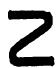
\includegraphics[keepaspectratio]{images/part001_b5dea1c7.jpg}}

On the set \(\mathbf{R}^n\) , we shall have to consider on the one hand its (additive) topological group structure and on the other hand its vector space structure over the field \(\mathbf{R}\) (Chapter VI, § 1, no. 3). Given a subset \(\mathbf{A}\) of \(\mathbf{R}^n\) , we may envisage the subgroup of \(\mathbf{R}^n\) generated by \(\mathbf{A}\) (the set of all linear combinations of points of \(\mathbf{A}\) , with integer coefficients) and also the vector subspace generated by \(\mathbf{A}\) (the set of all linear combinations of points of \(\mathbf{A}\) , with real coefficients); these two notions must be carefully distinguished. In accordance with the definitions made in algebra, the rank of \(\mathbf{A}\) is the dimension of the vector subspace \(\mathbf{V}\) of \(\mathbf{R}^n\) generated by \(\mathbf{A}\) ; to say that \(\mathbf{A}\) is of rank \(p\) is therefore equivalent to saying that there are \(p\) points \(x_i \in \mathbf{A}\) which form a free system with respect to the field \(\mathbf{R}\) (in other words, the relation \(\sum_{i} t_i x_i = 0\) , where the \(t_i\) are real, implies \(t_i = 0\) for each \(i\) ) and form a basis of \(\mathbf{V}\) (which means that every point of \(\mathbf{V}\) is a linear combination of the \(x_i\) with real coefficients).

In what follows we shall also have to make use of the notion of a system of points of \(\mathbf{R}^n\) which are free with respect to the field \(\mathbf{Q}\) of rational numbers; such a system is a finite subset \((\pmb{x}_i)\) of \(\mathbf{R}^n\) such that the relation \(\sum_{i} r_i x_i = 0\) , where the \(r_i\) are rational numbers (or integers --- it comes to the same thing), implies that \(r_{i}=0\) for each i. This notion must be carefully distinguished from that of a free system with respect to R: every system which is free with respect to R is free with respect to Q, but the converse is false (for example, the numbers 1 and \(\sqrt{2}\) in R form a free system with respect to Q, but not a free system with respect to R). Whenever we speak of a free system without qualification, we shall always mean a free system with respect to R. It is therefore necessary to distinguish on \(R^{n}\) the vector space structure with respect to R from the vector space structure with respect to Q; in particular, the vector subspace with respect to Q generated by a subset A of \(R^{n}\) is the set U of all linear combinations of A with rational coefficients; it is contained in the vector subspace V (with respect to R) generated by A, but is in general distinct from V. The dimension of U (with respect to Q) is called the rational rank of A; it is at least equal to the rank of A defined above (the dimension of V with respect to R); it may be infinite if A is an infinite set, while the rank of any non-empty subset of \(R^{n}\) is always \(\leqslant n\) ; in particular, the rational rank of any uncountable subset of \(R^{n}\) is always infinite, because any finite-dimensional vector space over Q is countable.

\pandocbounded{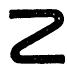
\includegraphics[keepaspectratio]{images/part001_3371d17f.jpg}}

In this section we shall first determine the structure of the closed subgroups of the additive group \(R^{n}\) .

\subsection{\texorpdfstring{DISCRETE SUBGROUPS OF \(\mathbf{R}^n\)}{DISCRETE SUBGROUPS OF R TO THE N}}

We have seen in Chapter V (§ 1, no. 1, Proposition 1) that the only closed subgroups of R, other than R itself, are the discrete subgroups, generated by a single element. We shall begin by considering the discrete subgroups of \(\mathbf{R}^n\) .

First of all, the subgroup of \(\mathbf{R}^n\) generated by \(p\) vectors ( \(p \leqslant n\) ) of the canonical basis (Chapter VI, § 1, no. 3) of \(\mathbf{R}^n\) is a discrete group isomorphic to the product \(\mathbf{Z}^p\) of \(p\) groups which are equal to \(\mathbf{Z}\) . More generally, consider the subgroup \(\mathbf{G}\) generated by \(p\) points \(a_i\) ( \(i \leqslant i \leqslant p\) ) which form a free system. There is a bijective linear mapping of \(\mathbf{R}^n\) onto itself which maps \(a_i\) to \(e_i\) ( \(i \leqslant i \leqslant p\) ); since such a mapping is an automorphism of the topological group \(\mathbf{R}^n\) , \(\mathbf{G}\) is isomorphic as a topological group to the subgroup generated by the \(e_i\) ( \(i \leqslant i \leqslant p\) ) and is therefore a discrete subgroup of rank \(p\) isomorphic to \(\mathbf{Z}^p\) .

The structure of the group \(Z^{p}\) , and hence that of G, has been studied in algebra. We recall the main results of this study. The bases of G with respect to the ring Z are systems of p points

\[
\boldsymbol {b} _ {i} = \sum_ {j = 1} ^ {p} r _ {i j} \boldsymbol {a} _ {j},
\]

where the \(r_{ij}\) are integers such that the determinant \(\det(r_{ij})\) is equal to +1 or -1. Every subgroup H of G is discrete and of rank \(q \leqslant p;\) furthermore, if \(H\) is a given subgroup of rank \(q\) , there exists a free system of \(p\) points \(b_i\) ( \(i \leqslant i \leqslant p\) ) which generates \(G\) , and a system of \(q\) points \(c_i\) ( \(i \leqslant i \leqslant q\) ) which generates \(H\) , such that we have \(c_i = e_i b_i\) for \(i \leqslant i \leqslant q\) , where the \(e_i\) are integers (the invariant factors of \(H\) with respect to \(G\) ) such that

\[
e _ {i + 1} \equiv o (\mathrm{mod} e _ {i}) \quad \text { for } \quad i \leqslant i \leqslant q - i.
\]

The quotient group G/H is a discrete group isomorphic to \(Z^{p-q} \times F\) , where F is a finite abelian group, the direct product of q cyclic subgroups of respective orders \(e_{1}, \ldots, e_{q}\) .

We shall show now that the discrete subgroups of \(\mathbf{R}^n\) which we have just been considering are the only ones that exist.

PROPOSITION 1. Let G be a discrete subgroup of \(\mathbf{R}^n\) of rank \(p\) , let \((\boldsymbol{a}_i)_{1 \leqslant i \leqslant p}\) be a free system of \(p\) points of G, and let P be the closed parallelotope with centre o and basis vectors \(\boldsymbol{a}_i\) (Chapter VI, § 1, no. 3). Then the set G ∩ P is finite and generates G, and every point of G is a linear combination of the \(\boldsymbol{a}_i\) with rational coefficients.

G ∩ P is compact and discrete, hence finite. Let x be any point of G; it is equal to a linear combination \(\sum_{i=1}^{p} t_{i}a_{i}\) of the \(a_{i}\) with real coefficients. For each integer m \textgreater{} 0, consider the point

\[
z _ {m} = m x - \sum_ {i = 1} ^ {p} [ m t _ {i} ] a _ {i} = \sum_ {i = 1} ^ {p} (m t _ {i} - [ m t _ {i} ]) a _ {i} (*);
\]

it belongs to G, and since \(o \leqslant mt_{i} - [mt_{i}] < 1\) , it lies in P. Hence, first, \(x = z_{1} + \sum_{i=1}^{p} [t_{i}] a_{i}\) , so that G is generated by \(G \cap P\) ; and secondly, since \(G \cap P\) is finite, there exist two distinct integers h, k such that \(z_{h} = z_{k}\) , so that \((h - k)t_{i} = [ht_{i}] - [kt_{i}]\) less \((1 \leqslant i \leqslant p)\) , and therefore the \(t_{i}\) are rational numbers.

COROLLARY. Let \((\pmb{a}_i)_{1\leqslant i\leqslant p}\) be a free system of \(p\) points of \(\mathbf{R}^n\) and let

\[
\boldsymbol {b} = \sum_ {i = 1} ^ {p} t _ {i} \boldsymbol {a} _ {i}
\]

be a linear combination of the \(a_{i}\) , with real coefficients. Then the subgroup G of \(R^{n}\) generated by the \(p + i\) points \(a_{1}, a_{2}, \ldots, a_{p}\) and b is discrete if and only if the numbers \(t_{i}\) are rational.

Proposition 1 shows that the condition is necessary. Also it is sufficient, for if it is satisfied we can write \(t_i = m_i / d\) , where \(d\) and the \(m_i\) are integers ( \(i \leqslant i \leqslant p\) ); \(b\) is therefore a linear combination, with integer coefficients, of the \(p\) points ( \(\mathrm{I} / d\) ) \(a_i\) ; hence \(G\) is a subgroup of the discrete group generated by these \(p\) points, and so is itself discrete.

The result of Proposition 1 can be expressed as follows: if q points \(x_{i}\) ( \(i \leqslant i \leqslant q\) ) of a discrete subgroup G of \(R^{n}\) form a system which is dependent with respect to R, then they form a system which is dependent with respect to Q. It follows immediately that the rational rank of a discrete subgroup of \(R^{n}\) is equal to its rank.

The Corollary to Proposition 1, applied to the case where the \(a_{i}\) are the \(n\) vectors \(\pmb{e}_{i}\) of the canonical basis of \(\mathbf{R}^{n}\) , gives us the following proposition:

PROPOSITION 2 (Kronecker). Let \(\theta_{1}, \theta_{2}, \ldots, \theta_{n}\) be \(n\) real numbers. In order that, for each \(\varepsilon > 0\) , there exist an integer \(q\) and \(n\) integers

\[
p _ {i} \quad (\mathrm{I} \leqslant i \leqslant n)
\]

such that

\[
\left| q \theta_ {i} - p _ {i} \right| \leqslant \varepsilon \quad (\mathrm{I} \leqslant i \leqslant n),
\]

where the left-hand side of at least one of these inequalities does not vanish, it is necessary and sufficient that at least one of the \(\theta_{i}\) be irrational.

THEOREM 1. Every discrete subgroup G of \(\mathbf{R}^n\) , of rank equal to \(p\) , is generated by a free system of \(p\) points.

By virtue of the properties of groups isomorphic to \(Z^{p}\) recalled earlier, it is enough to show that G is a subgroup of a discrete group generated by a free system of p points. Now since G is of rank p there exists a free system of p points \(a_{i}\) ( \(1 \leqslant i \leqslant p\) ) of G such that every \(x \in G\)

is equal to a linear combination \(\sum_{i=1}^{p} t_i a_i\) of the \(a_i\) with real coefficients;

since G is discrete, Proposition 1 shows that the \(t_i\) are rational. Furthermore, Proposition 1 shows that G is generated by a finite number of points; since these points are linear combinations of the \(\boldsymbol{a}_i\) with rational coefficients, there exists an integer \(d\) such that they are linear combinations with integer coefficients of the \(p\) points \((\mathrm{I}/d)\boldsymbol{a}_i = \boldsymbol{a}_i'\) . It follows that G is a subgroup of the group generated by the \(\boldsymbol{a}_i'\) .

Theorem 1 can also be proved without recourse to the theory of invariant factors (cf.~Exercise 1).

Discrete subgroups of \(R^{n}\) which are of rank n are also called lattices in \(R^{n}\) .

\subsection{\texorpdfstring{CLOSED SUBGROUPS OF \(\mathbf{R}^n\)}{CLOSED SUBGROUPS OF R TO THE N}}

We know already of two types of closed subgroups of \(\mathbf{R}^n\) ; on the one hand, the vector subspaces of \(\mathbf{R}^n\) , which are isomorphic to the groups \(\mathbf{R}^p\) ( \(p \leqslant n\) ) (Chapter IV, § 1, no. 4, Proposition 2); on the other hand, the discrete subgroups (Chapter III, § 2, no. 1, Proposition 5) which are isomorphic to groups \(\mathbf{Z}^q\) ( \(q \leqslant n\) ), as we have just seen. We shall now determine the structure of an arbitrary closed subgroup of \(\mathbf{R}^n\) by showing that such a subgroup is isomorphic to a product of the form

\[
\mathbf {R} ^ {p} \times \mathbf {Z} ^ {q} \quad \text { where } \quad \mathrm{o} \leqslant p + q \leqslant n.
\]

The proof rests on the following proposition:

PROPOSITION 3. Every non-discrete closed subgroup of \(\mathbf{R}^n\) contains a line passing through o.

Let \((\pmb{x}_p)_{p\in \mathbb{N}}\) be an infinite sequence of points of \(\mathbf{G}\) such that \(\pmb{x}_p\neq 0\) and \(\lim_{p\to \infty}\pmb{x}_p = 0\) ; by hypothesis such a sequence exists. Let \(\mathbf{P}\) be an open cube with centre \(0\) , containing the \(\pmb{x}_p\) . Let \(k_{p}\) denote the largest integer \(h > 0\) such that \(h\pmb{x}_p\in \mathrm{P}\) (since \(\mathbf{P}\) is a bounded box and \(\pmb{x}_p\neq 0\) , the existence of \(k_{p}\) follows from Archimedes' axiom). The points \(k_{p}\pmb{x}_{p}\) lie in a compact set \(\overline{\mathrm{P}}\) , hence the sequence \((k_{p}\pmb{x}_{p})_{p\in \mathbb{N}}\) has a cluster point \(\pmb {a}\in \overline{\mathrm{P}}\) . If \(||k_p\pmb {x}_p - \pmb {a}||\leqslant \varepsilon\) , we have

\[
\left| \left| \left(k _ {p} + \mathrm{I}\right) x _ {p} - a \right| \right| \leqslant \varepsilon + \left| \left| x _ {p} \right| \right|,
\]

and since \(\lim_{p\to \infty}\boldsymbol{x}_p = 0\) , it follows that \(\boldsymbol{a}\) is also a cluster point of the sequence \(((k_p + 1)x_p)\) , whose points belong to the closed set \(\mathfrak{C}P\) , by definition of \(k_{p}\) ; hence \(\boldsymbol{a} \in \overline{\mathrm{P}} \cap \mathfrak{C}P\) (the frontier of P, Fig. 5), which implies \(\boldsymbol{a} \neq 0\) . Moreover, since G is closed, we have \(\boldsymbol{a} \in \mathrm{G}\) . Let \(t\) be any real number; since \(|tk_p - [tk_p]| < 1\) , the relation \(||k_p x_p - a|| \leqslant \varepsilon\) implies that \(||[tk_p]x_p - ta|| \leqslant |t| \varepsilon + ||x_p||\) ; since \(\lim_{p \to \infty} x_p = 0\) , \(ta\) is a

\pandocbounded{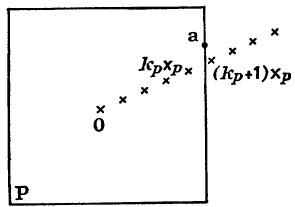
\includegraphics[keepaspectratio]{images/part001_2a0a1c84.jpg}}\\
Figure 5.

\pandocbounded{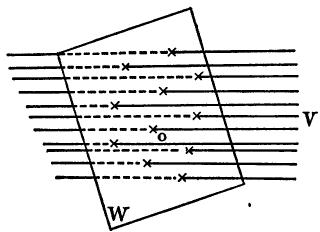
\includegraphics[keepaspectratio]{images/part001_3dc381fa.jpg}}\\
Figure 6.

cluster point of the sequence \(([tk_p]x_p)\) ; but the points of this sequence belong to G, and consequently \(ta \in G\) , since G is closed. This completes the proof.

THEOREM 2. Let G be a closed subgroup of \(\mathbf{R}^n\) , of rank \(r\) ( \(0 \leqslant r \leqslant n\) ). Then there is a largest vector subspace V contained in G; for every vector subspace W complementary to V, W ∩ G is discrete and G is the direct sum of V and W ∩ G.

Let us first establish the existence of V by showing that the union of all the lines through o which lie in G is a vector subspace: indeed, the vector subspace generated by the union of these lines is the same as the subgroup they generate. The group G is the direct sum of V and W ∩ G; for if \(x \in G\) , we have \(x = y + z\) where \(y \in V\) and \(z \in W\) ; since \(V \subset G\) , \(z = x - y \in G\) and therefore \(z \in W \cap G\) . It remains to show that \(W \cap G\) is discrete; this follows from Proposition 3, since \(W \cap G\) is a closed subgroup which contains no lines, by reason of the definition of V.

If \(G \neq V\) , we may say that G is the union of a countable infinity of linear varieties, parallel to V and passing through the points of the discrete group \(W \cap G\) (Fig. 6).

If \(p\) is the dimension of the vector subspace \(\mathbf{V}\) , we have \(p \leqslant r\) , and \(\mathbf{W} \cap \mathbf{G}\) is a discrete group of rank \(r - p\) .

COROLLARY 1. There exists a basis \((\pmb{a}_i)_{1\leqslant i\leqslant n}\) of \(\mathbf{R}^n\) , such that

\[
\boldsymbol {a} _ {i} \in \mathrm{G} \quad (\mathrm{I} \leqslant i \leqslant r), \quad \boldsymbol {a} _ {i} \in \mathrm{V} \quad (\mathrm{I} \leqslant i \leqslant p)
\]

and such that \(\mathbf{G}\) is the set of points \(\sum_{i=1}^{p} t_i a_i + \sum_{j=p+1}^{r} n_j a_j\) , where the \(t_i\) take all real values and the \(n_j\) take all integer values.

This follows from Theorem 2, and Theorem 1 of no. 1 applied to the discrete group \(W \cap G\) .

COROLLARY 2. There exists an automorphism of \(\mathbf{R}^n\) which maps \(\mathbf{G}\) onto the group \(\mathbf{G}'\) , isomorphic to \(\mathbf{R}^p \times \mathbf{Z}^{r-p}\) , which is the direct sum of the vector subspace generated by \(e_1, e_2, \ldots, e_p\) and the (discrete) additive subgroup generated by \(e_{p+1}, e_{p+2}, \ldots, e_r\) .

This is an immediate consequence of Corollary 1. Corollary 2 of Theorem 2 shows that a closed subgroup G of \(R^{n}\) is completely determined up to isomorphism by two integers \(\geqslant 0\) : its rank, which we denote by \(r(\mathbf{G})\) , and the dimension of the largest vector subspace contained in G, which we call the dimension of G and denote by \(d(\mathbf{G})\) .

The only conditions which these integers have to satisfy are the inequalities \(o \leqslant d(\mathbf{G}) \leqslant r(\mathbf{G}) \leqslant n\) .

\subsection{ASSOCIATED SUBGROUPS}

Let \(\mathbf{G}\) be an arbitrary subgroup (closed or not) of \(\mathbf{R}^n\) . Consider the set \(\mathbf{G}^*\) of points \(\boldsymbol{u} = (u_i) \in \mathbf{R}^n\) such that, for all \(\boldsymbol{x} = (x_i) \in \mathbf{G}\) , the number \((\boldsymbol{u}| \boldsymbol{x}) = \sum_{i=1}^{n} u_i x_i\) is an integer. It is immediately seen that \(\mathbf{G}^*\) is a subgroup of \(\mathbf{R}^n\) ; it is called the subgroup associated with \(\mathbf{G}(*)\) . If \(\mathbf{G}\) and \(\mathbf{H}\) are two subgroups of \(\mathbf{R}^n\) such that \(\mathbf{H} \subset \mathbf{G}\) , it is clear that \(\mathbf{G}^* \subset \mathbf{H}^*\) .

PROPOSITION 4. The subgroup \(\mathbf{G}^*\) associated with a subgroup \(\mathbf{G}\) of \(\mathbf{R}^n\) is closed, and we have \((\overline{\mathbf{G}})^* = \mathbf{G}^*\) .

For each \(x \in G\) , let \(f_x(u)\) denote \((u|x)\) ; \(f_x\) is a linear form, therefore continuous. Since \(G^*\) is the intersection of the sets \(f_x^{-1}(Z)\) as \(x\) runs through \(G\) , and since each of these sets is closed, it follows that \(G^*\) is closed. On the other hand, if \(u \in G^*\) , we have \((u|x) \in Z\) for all \(x \in G\) , and therefore, as \(Z\) is closed in \(R\) , \((u|y) \in Z\) for all \(y \in \overline{G}\) ; thus \(u \in (G)^*\) . But we have \((\overline{G})^* \subset G^*\) (since \(G \subset \overline{G}\) ), so that \((\overline{G})^* = G^*\) .

Consider the structure of \(\mathbf{G}^*\) when \(\mathbf{G}\) is closed. By Corollary 1 to Theorem 2 of no. 2, there exists a base \((\pmb{a}_i)_{\mathbf{1} \leqslant i \leqslant n}\) of \(\mathbf{R}^n\) such that \(\mathbf{G}\) coincides with the set of points

\[
\boldsymbol {x} = \sum_ {i = 1} ^ {p} t _ {i} \boldsymbol {a} _ {i} + \sum_ {j = p + 1} ^ {p + q} n _ {j} \boldsymbol {a} _ {j},
\]

where the \(t_i\) take all real values and the \(n_j\) take all integer values. Hence \((\boldsymbol{u}|\boldsymbol{x})\) is an integer for all these points \(\boldsymbol{x}\) if and only if \((\boldsymbol{u}|\boldsymbol{a}_i) = 0\) for \(1 \leqslant i \leqslant p\) and \((\boldsymbol{u}|\boldsymbol{a}_i)\) is an integer for \(p + 1 \leqslant i \leqslant p + q\) . Let us denote by \((\boldsymbol{a}_i')_{1 \leqslant i \leqslant n}\) the basis of \(\mathbf{R}^n\) such that \((\boldsymbol{a}_i'|\boldsymbol{a}_j) = 0\) for \(i \neq j\) and

\[
\left(\boldsymbol {a} _ {i} ^ {\prime} \mid \boldsymbol {a} _ {i}\right) = \mathrm{I} \quad \text { for } \quad \mathrm{I} \leqslant i \leqslant n
\]

{[}the basis `` dual '' to \((a_{i})\) {]}; if we put \(u = \sum_{i=1}^{n} u_{i} a_{i}^{\prime}\) , it is clear that the points \(u \in G^{*}\) are characterized by the following conditions: \(u_{i} = 0\) for \(i \leqslant i \leqslant p\) , and \(u_{i} \in Z\) for

\[
p + \mathrm{i} \leqslant i \leqslant p + q;
\]

hence \(G^{*}\) is the direct sum of a vector subspace W with a basis consisting of the \(a_{i}^{\prime}\) such that \(p + q + i \leqslant i \leqslant n\) , and a discrete subgroup generated by the \(a_{i}^{\prime}\) such that \(p + i \leqslant i \leqslant p + q\) . In other words:

PROPOSITION 5. For every closed subgroup G of \(\mathbf{R}^n\) ,

\[
r (\mathbf {G} ^ {*}) = n - d (\mathbf {G}) \quad a n d \quad d (\mathbf {G} ^ {*}) = n - r (\mathbf {G}).
\]

Let us apply the same reasoning to \(\mathbf{G}^*\) . Observing that the basis dual to \((\pmb{a}_i')\) is \((\pmb{a}_i)\) , we see that:

PROPOSITION 6. For every subgroup \(\mathbf{G}\) of \(\mathbf{R}^n\) , we have \((\mathbf{G}^*)^* = \overline{\mathbf{G}}\) .

COROLLARY. A point x lies in the closure of a subgroup G of \(R^{n}\) if and only if \((u|x)\) is an integer for all \(u \in R^{n}\) such that \((u|y)\) is an integer for all \(y \in G\) .

Let us apply this characterization of points lying in the closure of a subgroup \(\mathbf{G}\) to the case of the subgroup \(\mathbf{G}\) generated by the \(n\) vectors \(\boldsymbol{e}_j\) of the canonical basis ( \(\mathrm{i} \leqslant j \leqslant n\) ) and by an arbitrary number \(m\) of points \(\boldsymbol{a}_i\) ( \(\mathrm{i} \leqslant i \leqslant m\) ) of \(\mathbf{R}^n\) . To say that \((\boldsymbol{u}|\boldsymbol{e}_j)\) is an integer for \(\mathrm{i} \leqslant j \leqslant n\) means that the \(n\) coordinates of \(\boldsymbol{u}\) are integers; therefore:

PROPOSITION 7 (Kronecker). Let \(\boldsymbol{a}_i = (a_{ji})\) ( \(i \leqslant i \leqslant m\) , \(i \leqslant j \leqslant n\) ) be \(m\) points of \(\mathbf{R}^n\) and let \(\boldsymbol{b} = (b_j)\) ( \(i \leqslant j \leqslant n\) ) be a point of \(\mathbf{R}^n\) . In order that, for each \(\varepsilon > 0\) , there exist \(m\) integers \(g_i\) ( \(i \leqslant i \leqslant m\) ) and \(n\) integers \(p_j\) ( \(i \leqslant j \leqslant n\) ) such that

\[
\left| q _ {1} a _ {1 j} + q _ {2} a _ {2 j} + \dots + q _ {m} a _ {m j} - p _ {j} - b _ {j} \right| \leqslant \varepsilon \quad (\mathrm{I} \leqslant j \leqslant n)
\]

it is necessary and sufficient that, for each finite sequence \((r_j)\) ( \(1 \leqslant j \leqslant n\) ) of \(n\) integers such that the \(m\) numbers \(\sum_{j=1}^{n} a_{ij} r_j\) ( \(1 \leqslant i \leqslant m\) ) are all integers, the number \(\sum_{j=1}^{n} b_j r_j\) should also be an integer.

COROLLARY 1. In order that, for each \(\boldsymbol{x} = (x_{j}) (\mathrm{I} \leqslant j \leqslant n)\) and each \(\varepsilon > 0\) , there exist m integers \(q_{i} (\mathrm{I} \leqslant i \leqslant m)\) and n integers

\(p_j\) (1 \(\leqslant j\leqslant n\) ) such that

\[
\left| q _ {1} a _ {1 j} + q _ {2} a _ {2 j} + \dots + q _ {m} a _ {m j} - p _ {j} - x _ {j} \right| \leqslant \varepsilon \quad (\mathrm{I} \leqslant j \leqslant n)
\]

it is necessary and sufficient that there exist no finite sequence \((r_j)\) of \(n\) integers, not all zero, such that each of the \(m\) numbers \(\sum_{j=1}^{n} a_{ij} r_j\) is an integer. For if \(G\) is dense in \(\mathbf{R}^n\) , that is if \(\overline{\mathbf{G}} = \mathbf{R}^n\) , then \(\mathbf{G}^* = \{o\}\) , and conversely.

In particular \((m = \mathrm{i})\) :

COROLLARY 2. Let \(\theta_{1},\theta_{2},\ldots ,\theta_{n}\) be \(n\) real numbers. In order that, given any \(n\) real numbers \(x_{1},x_{2},\ldots ,x_{n}\) and a real number \(\varepsilon >0\) , there should exist an integer \(q\) and \(n\) integers \(p_j\) such that

\[
\left| q \theta_ {j} - p _ {j} - x _ {j} \right| \leqslant \varepsilon \quad (\mathrm{I} \leqslant j \leqslant n)
\]

it is necessary and sufficient that there exist no relation of the form \(\sum_{j=1}^{n} r_j \theta_j = h\) , where the \(r_j\) are \(n\) integers not all zero, and \(h\) is an integer {[}which implies, in particular, that the \(\theta_j\) and the ratios \(\theta_j / \theta_k\) ( \(j \neq k\) ) must be irrational{]}.

We may interpret this result as follows: for each integer \(q \in Z\) , let \(x_{q}\) denote the point with coordinates \(q\theta_{j} - [q\theta_{j}]\) ( \(i \leqslant j \leqslant n\) ); then Corollary 2 gives a necessary and sufficient condition for the set of points \(x_{q}\) to be dense in the cube which is the product of n intervals {[}0, i{]} in the factors of \(R^{n}\) .

PROPOSITION 8. If \(G_{1}\) , \(G_{2}\) are any closed subgroups of \(R^{n}\) , we have

\[
(\mathrm{G} _ {1} + \mathrm{G} _ {2}) ^ {*} = \mathrm{G} _ {1} ^ {*} \cap \mathrm{G} _ {2} ^ {*} \quad a n d \quad (\mathrm{G} _ {1} \cap \mathrm{G} _ {2}) ^ {*} = \mathrm{G} _ {1} ^ {*} + \mathrm{G} _ {2} ^ {*}.
\]

The real number \((\pmb{u}|\pmb{x} + \pmb{y})\) is an integer for all \(\pmb{x} \in \mathbf{G}_1\) and all \(\pmb{y} \in \mathbf{G}_2\) if and only if \((\pmb{u}|\pmb{x})\) is an integer for all \(\pmb{x} \in \mathbf{G}_1\) and \((\pmb{u}|\pmb{y})\) is an integer for all \(\pmb{y} \in \mathbf{G}_2\) , because \((\pmb{u}|\pmb{x} + \pmb{y}) = (\pmb{u}|\pmb{x}) + (\pmb{u}|\pmb{y})\) ; hence

\[
(\mathrm{G} _ {1} + \mathrm{G} _ {2}) ^ {*} = \mathrm{G} _ {1} ^ {*} \cap \mathrm{G} _ {2} ^ {*}
\]

for any two subgroups \(G_{1}\) , \(G_{2}\) of \(R^{n}\) . If now we suppose that \(G_{1}\) and \(G_{2}\) are closed, we have \((\mathbf{G}_{1}^{*} + \mathbf{G}_{2}^{*})^{*} = \mathbf{G}_{1} \cap \mathbf{G}_{2}\) by Proposition 6; hence, taking the associated subgroups and applying Proposition 6 again, \((\mathbf{G}_{1} \cap \mathbf{G}_{2})^{*} = \overline{\mathbf{G}_{1}^{*} + \mathbf{G}_{2}^{*}}\) .

Remark. Let \(\mathbf{G}_1, \mathbf{G}_2\) be two lattices in \(\mathbf{R}^n\) (no. 1) such that \(\mathbf{G}_2 \subset \mathbf{G}_1\) ; then (Proposition 5) \(\mathbf{G}_1^*\) and \(\mathbf{G}_2^*\) are lattices in \(\mathbf{R}^n\) such that \(\mathbf{G}_1^* \subset \mathbf{G}_2^*\) . We have seen in no. 1 that there is an integer \(m > 0\) such that \(m\mathbf{G}_1 \subset \mathbf{G}_2\) ;

consequently for \(x \in G_1\) and \(u \in G_2^*\) we have \(m(u|x) \in Z\) and therefore \((u|x) \in Q\) . If \(x \in G_2\) and \(u \in G_2^*\) , or if \(x \in G_1\) and \(u \in G_1^*\) , we have \((u|x) \in Z\) by definition. Consequently on passing to the quotients the \(Z\) -bilinear mapping \((x, u) \to (u|x)\) of \(G_1 \times G_2^*\) into \(Q\) defines a \(Z\) -bilinear mapping \(B\) of \((G_1/G_2) \times (G_2^*/G_1^*)\) into \(Q/Z\) . Moreover, it is clear that if \(\bar{x}_0 \in G_1/G_2\) (resp. \(\bar{u}_0 \in G_2^*/G_1^*\) ) is such that, for each \(\bar{u} \in G_2^*/G_1^*\) (resp. for each \(\bar{x} \in G_1/G_2\) ) we have

\[
\mathrm{B} (\overline {{{\boldsymbol {x}}}} _ {0}, \boldsymbol {u}) = \mathrm{o} \quad [ \text { resp. } \mathrm{B} (\overline {{{\boldsymbol {x}}}}, \overline {{{\boldsymbol {u}}}} _ {0}) = \mathrm{o} ],
\]

then necessarily \(\overline{\mathbf{x}}_0 = \mathbf{o}\) (resp. \(\overline{\mathbf{u}}_0 = \mathbf{o}\) ). It follows that there is a \(\mathbf{Z}\) -linear bijection \(h\) of \(\mathrm{G}_2^* / \mathrm{G}_1^*\) onto the dual of \(\mathrm{G}_1 / \mathrm{G}_2\) , such that \(\langle \overline{\mathbf{x}}, h(\overline{\mathbf{u}}) \rangle = \mathrm{B}(\overline{\mathbf{x}}, \overline{\mathbf{u}})\) for \(\overline{\mathbf{x}} \in \mathrm{G}_1 / \mathrm{G}_2\) and \(\overline{\mathbf{u}} \in \mathrm{G}_2^* / \mathrm{G}_1^*\) ; in particular, the finite groups \(\mathrm{G}_1 / \mathrm{G}_2\) and \(\mathrm{G}_2^* / \mathrm{G}_1^*\) are isomorphic.

\subsection{\texorpdfstring{HAUSDORFF QUOTIENT GROUPS OF \(R^{n}\)}{HAUSDORFF QUOTIENT GROUPS OF R TO THE N}}

Every Hausdorff quotient group of \(\mathbf{R}^n\) is of the form \(\mathbf{R}^n/\mathbf{H}\) , where \(\mathbf{H}\) is a closed subgroup of \(\mathbf{R}^n\) (Chapter III, § 2, no. 6, Proposition 18). By Corollary 2, Theorem 2 of no. 3, there exists an automorphism \(f\) of \(\mathbf{R}^n\) which transforms \(\mathbf{H}\) into a subgroup \(\mathbf{H}'\) , the direct sum of a vector subspace generated by \(p\) of the vectors \(\boldsymbol{e}_i\) of the canonical basis and the discrete group generated by \(q\) of the \(n-p\) remaining vectors

\[
\boldsymbol {e} _ {i}, \quad \mathrm{o} \leqslant p + q \leqslant n.
\]

Passing to the quotients, \(f\) induces an isomorphism of \(\mathbf{R}^n / \mathbf{H}\) onto \(\mathbf{R}^n / \mathbf{H}'\) (Chapter III, § 2, no. 8, Remark 3); now, \(\mathbf{R}^n / \mathbf{H}'\) is isomorphic to \(\mathbf{R}^{n - p - q} \times \mathbf{T}^q\) (Chapter III, § 2, no. 9, Corollary to Proposition 26). Consequently:

PROPOSITION 9. Every Hausdorff quotient group of \(\mathbf{R}^{n}\) is isomorphic to a product group \(\mathbf{R}^{h} \times \mathbf{T}^{k}\) ( \(0 \leqslant h + k \leqslant n\) ).

The product space \(\mathbf{T}^n\) (and, by abuse of language, the topological group \(\mathbf{T}^n\) ) is called the \(n\) -dimensional torus; by Proposition 4 of Chapter V, §1, no. 2, \(\mathbf{T}^n\) is compact, connected and locally connected.

Furthermore, if C denotes a closed cube of side 1 in \(R^{n}\) , \(T^{n}\) is homeomorphic to the quotient space of C by the equivalence relation `` \(x_{i} \equiv y_{i} \pmod{1}\) ( \(1 \leqslant i \leqslant n\) )'' between the points \(\boldsymbol{x} = (\boldsymbol{x}_{i})\) and \(\boldsymbol{y} = (\boldsymbol{y}_{i})\) of C. Thus \(T^{n}\) is formed from the cube C by ``identification of opposite faces''.

PROPOSITION 10. The topological group \(\mathbf{T}^n\) is locally isomorphic to \(\mathbf{R}^n\) . For \(\mathbf{T}^n = (\mathbf{R}/\mathbf{Z})^n\) is isomorphic to \(\mathbf{R}^n/\mathbf{Z}^n\) (Chapter III, § 2, no. 9, Corollary to Proposition 26) and \(\mathbf{Z}^n\) is a discrete subgroup of \(\mathbf{R}^n\) (Chapter III, § 2, no. 6, Proposition 19).

It follows that the groups \(\mathbf{R}^p\times \mathbf{T}^{n - p}\) are all locally isomorphic to \(\mathbf{R}^n\) \((\mathrm{o}\leqslant p\leqslant n)\) ; in § 2, no. 2, we shall see that they are the only connected groups which have this property.

\subsection{\texorpdfstring{SUBGROUPS AND QUOTIENT GROUPS OF \(T^{n}\)}{SUBGROUPS AND QUOTIENT GROUPS OF T TO THE N}}

Let us identify \(\mathbf{T}^n\) with \(\mathbf{R}^n/\mathbf{Z}^n\) , and let \(\varphi\) be the canonical homomorphism of \(\mathbf{R}^n\) onto \(\mathbf{R}^n/\mathbf{Z}^n\) . Every subgroup of \(\mathbf{T}^n\) is of the form \(\mathbf{G} = \varphi(\mathbf{H})\) where \(\mathbf{H}\) is a subgroup of \(\mathbf{R}^n\) which contains \(\mathbf{Z}^n\) and is isomorphic to \(\mathbf{H}/\mathbf{Z}^n\) (Chapter III, § 2, no. 7, Proposition 20); for \(\mathbf{G}\) to be closed in \(\mathbf{T}^n\) it is necessary and sufficient for \(\mathbf{H}\) to be closed in \(\mathbf{R}^n\) (Chapter I, § 3, no. 4). Thus in order to find the closed subgroups of \(\mathbf{T}^n\) we have to determine all the closed subgroups \(\mathbf{H}\) of \(\mathbf{R}^n\) which contain \(\mathbf{Z}^n\) ; to do this we shall use Proposition 6 of no. 3, and we start by determining the subgroup \(\mathbf{H}^*\) associated with \(\mathbf{H}\) . Since \(\mathbf{Z}^n\) is associated with itself, we have \(\mathbf{H}^* \subset \mathbf{Z}^n\) ; consequently (no. 1) there exists a basis \((\boldsymbol{a}_i)_{1 \leqslant i \leqslant n}\) of \(\mathbf{R}^n\) which generates \(\mathbf{Z}^n\) , and a basis of \(\mathbf{H}^*\) (with respect to the ring \(\mathbf{Z}\) ) consisting of \(p\) points \(\boldsymbol{b}_i\) ( \(1 \leqslant i \leqslant p\) ) such that \(\boldsymbol{b}_i = e_i \boldsymbol{a}_i\) ( \(1 \leqslant i \leqslant p\) ), where the \(e_i\) are integers satisfying the congruences \(e_{i+1} \equiv o (\text{mod } e_i)\) for \(1 \leqslant i \leqslant p - 1\) . Let \((\boldsymbol{a}_i')\) be the basis dual to \((\boldsymbol{a}_i)\) ; then \(\boldsymbol{u} = \sum_{i=1}^{n} u_i \boldsymbol{a}_i'\) belongs to \((\mathrm{H}^*)^* = \mathrm{H}\) if and only if \(u_i e_i \in \mathbf{Z}\) for \(1 \leqslant i \leqslant p\) ; in other words, \(\mathbf{H}\) is the direct sum of the vector subspace V generated by \(\boldsymbol{a}_{p+1}'\) , \ldots, \(\boldsymbol{a}_n'\) , and the discrete subgroup K generated by the \(p\) points

\[
e _ {i} ^ {- 1} \boldsymbol {a} _ {i} ^ {\prime} \quad (\mathrm{I} \leqslant i \leqslant p).
\]

On the other hand, \(\mathbf{Z}^n\) is the direct sum of \(\mathbf{V} \cap \mathbf{Z}^n\) and \(\mathbf{K} \cap \mathbf{Z}^n\) , because the \(a_i'\) ( \(i \leqslant i \leqslant n\) ) generate \(\mathbf{Z}^n\) . The quotient group \(\mathrm{H} / \mathbf{Z}^n\) is therefore isomorphic to \((\mathrm{V} / (\mathrm{V} \cap \mathbf{Z}^n)) \times (\mathrm{K} / (\mathrm{K} \cap \mathbf{Z}^n))\) (Chapter III, § 2, no. 9, Corollary to Proposition 26); \(\mathrm{V} / (\mathrm{V} \cap \mathbf{Z}^n)\) is isomorphic to \(\mathbf{T}^{n-p}\) , and \(\mathbf{K} / (\mathbf{K} \cap \mathbf{Z}^n)\) is a finite group, the direct sum of \(p\) cyclic groups of orders \(e_i\) , respectively ( \(i \leqslant i \leqslant p\) ) (cf.~no. 1).

Using the same notation, every Hausdorff quotient group of \(T^{n}\) is of the form \(\mathbf{T}^{n}/\varphi(\mathbf{H})\) and is isomorphic to \(R^{n}/H\) (Chapter III, § 2, no. 7, Corollary to Proposition 22); if W is the vector subspace generated by K, \(R^{n}/H\) is isomorphic to W/K (Chapter III, § 2, no. 9, Corollary to Proposition 26), i.e., to \(T^{p}\) . To sum up:

PROPOSITION 11. Every closed subgroup of \(\mathbf{T}^n\) is isomorphic to a group of the form \(\mathbf{T}^h \times \mathbf{F}\) ( \(0 \leqslant h \leqslant n\) ) where \(\mathbf{F}\) is a finite abelian group, such that the smallest number of cyclic subgroups of which \(\mathbf{F}\) is a direct sum is \(\leqslant n - h\) . Every Hausdorff quotient group of \(\mathbf{T}^n\) is isomorphic to a group of the form \(\mathbf{T}^h\) ( \(0 \leqslant h \leqslant n\) ).

In particular \((n = 1)\) :

COROLLARY. Every closed subgroup of T, other than T itself, is a finite cyclic group. Every Hausdorff quotient group of T, other than \(\{o\}\) , is isomorphic to T.

\subsection{PERIODIC FUNCTIONS}

DEFINITION 1. A function \(f\) , defined on \(\mathbf{R}^n\) , with values in an arbitrary set \(\mathbf{E}\) , is said to be periodic if there exists a point \(a \neq 0\) in \(\mathbf{R}^n\) such that

\[
f (\boldsymbol {x} + \boldsymbol {a}) = f (\boldsymbol {x})\tag{1}
\]

for all \(x \in R^{n}\) . If f is periodic, every point \(a \in R^{n}\) for which the relation (1) is an identity in x is called a period of f.

The set G of all periods of a periodic function f is clearly a subgroup (which by hypothesis does not consist of o alone) of the additive group \(R^{n}\) . If f is a continuous periodic mapping of \(R^{n}\) into a Hausdorff topological space E, its group of periods G is closed. For if \(G_{x}\) denotes the set of all \(a \in R^{n}\) such that \(f(x + a) = f(x)\) for a given point \(x \in R^{n}\) , then G is the intersection of the \(G_{x}\) as x runs through \(R^{n}\) , and each \(G_{x}\) is closed (Chapter I, § 8, no. 1, Proposition 2). Let V be the largest vector subspace contained in G (no. 2, Theorem 2); the function f is constant on every coset mod V; if W is a vector subspace complementary to V, then f is determined by its restriction to W. In other words (W being a topological group isomorphic to \(R^{p}\) for some p), the study of continuous periodic functions on \(R^{n}\) is reduced to the study of such functions whose group of periods G is discrete; if this group is of rank q, the function f is said to be q-ply periodic, and every free system of q points which generate G is called a principal system of periods of f.

If \((\boldsymbol{a}_{i})\) and \((\boldsymbol{b}_{i})\) are two principal systems of periods of f, we have seen (no. 1) that each can be obtained from the other by a linear transformation with integer coefficients and determinant \(\pm1\) .

Let \(\varphi\) be the canonical mapping of \(\mathbf{R}^n\) onto \(\mathbf{R}^n/\mathbf{G}\) ; to every mapping \(g\) of \(\mathbf{R}^n/\mathbf{G}\) into a set \(\mathbf{E}\) corresponds the function \(\dot{g}=g\circ\varphi\) , which is a periodic mapping of \(\mathbf{R}^n\) into \(\mathbf{E}\) , having a group of periods which contains G; and conversely every mapping of \(R^{n}\) into E which has a group of periods containing G is of this form, since it is compatible with the relation \(x \equiv y \pmod{G}\) (Set Theory, R, § 5, no. 7). In this way we define a bijective mapping \(g \to \dot{g}\) of the set of all mappings of \(R^{n}/G\) into E onto the set of all mappings of \(R^{n}\) into E whose group of periods contains G. For \(\dot{g}\) to be continuous (E being a topological space) it is necessary and sufficient that g should be continuous (Chapter I, § 3, no. 4, Proposition 6).

\section{\texorpdfstring{CONTINUOUS HOMOMORPHISMS OF \(\mathbf{R}^n\) AND ITS QUOTIENT GROUPS}{CONTINUOUS HOMOMORPHISMS OF R TO THE N AND ITS QUOTIENT GROUPS}}

\subsection{\texorpdfstring{CONTINUOUS HOMOMORPHISMS OF THE GROUP \(R^{m}\) INTO THE GROUP \(R^{n}\)}{CONTINUOUS HOMOMORPHISMS OF THE GROUP R TO THE M INTO THE GROUP R TO THE N}}

Every linear mapping (cf.~Chapter VI, § 1, no. 3) of \(\mathbf{R}^{m}\) into \(\mathbf{R}^{n}\) is evidently a continuous homomorphism of the additive group \(\mathbf{R}^{m}\) into the additive group \(\mathbf{R}^{n}\) . Conversely:

PROPOSITION 1. Every continuous homomorphism \(f\) of the additive group \(\mathbf{R}^m\) into the additive group \(\mathbf{R}^n\) is a linear mapping of \(\mathbf{R}^m\) into \(\mathbf{R}^n\) .

It is enough to show that \(f(tx) = tf(x)\) for all \(x \in \mathbf{R}^n\) and all \(t \in \mathbf{R}\) . The argument is the same as that of Proposition 5 of Chapter V, §1, no. 3 if we replace \(x\) by \(x\) and \(\mathbf{R}\) by \(\mathbf{R}^m\) .

\subsection{\texorpdfstring{LOCAL DEFINITION OF A CONTINUOUS HOMOMORPHISM OF \(R^{n}\) INTO A TOPOLOGICAL GROUP}{LOCAL DEFINITION OF A CONTINUOUS HOMOMORPHISM OF R TO THE N INTO A TOPOLOGICAL GROUP}}

Proposition 6 of Chapter V, § 1, no. 4 may be generalized to all the groups \(\mathbf{R}^n\) .

PROPOSITION 2. Let A be a parallelotope in \(\mathbf{R}^n\) which contains o; and let \(f\) be a continuous mapping of A into a topological group G (written multiplicatively) such that \(f(x + y) = f(x)f(y)\) for each pair of points \(x, y\) such that \(x \in A\) , \(y \in A\) and \(x + y \in A\) . Then there exists a unique continuous homomorphism of \(\mathbf{R}^n\) into G which extends \(f\) .

By the same reasoning as in Proposition 6 of Chapter V, §1, no. 4 we show that the homomorphism extending \(f\) , if it exists, is unique. Next, the subgroup \(G_1\) of \(G\) , generated by \(f(A)\) , is commutative; for if \(x\) and y are any two points of A, then \(\frac{1}{2}x\) , \(\frac{1}{2}y\) and \(\frac{1}{2}(x+y)\) belong to A, therefore

\[
f \left(\frac {1}{2} (\boldsymbol {x} + \boldsymbol {y})\right) = f \left(\frac {1}{2} \boldsymbol {x}\right) f \left(\frac {1}{2} \boldsymbol {y}\right) = f \left(\frac {1}{2} \boldsymbol {y}\right) f \left(\frac {1}{2} \boldsymbol {x}\right),
\]

which shows that \(f(\frac{1}{2} x)\) and \(f(\frac{1}{2} y)\) commute; therefore so do \(f(x) = (f(\frac{1}{2} x))^2\) and \(f(y) = (f(\frac{1}{2} y))^2\) , which proves the assertion.

Let \(a_1, a_2, \ldots, a_n\) be \(n\) non-zero vectors contained in \(A\) and proportional to the basis vectors of the parallelotope, and for each index \(i\) let \(D_i\) be the line through \(o\) and \(a_i\) , that is, the set of points \(ta_i\) as \(t\) runs through \(R\) . Let \(A_i\) be the set of all \(t \in R\) such that \(ta_i \in A\) ; then \(A_i\) is an interval of \(R\) containing \([o, i]\) , and the function

\[
f _ {i} (t) = f \left(t \boldsymbol {a} _ {i}\right)
\]

is defined and continuous on \(A_{i}\) and satisfies the relation

\[
f _ {i} (t + t ^ {\prime}) = f _ {i} (t) f _ {i} (t ^ {\prime})
\]

whenever \(t, t'\) and \(t + t'\) all belong to \(A_i\) . By Proposition 6 of Chapter V, §1, no. 4, there exists a continuous homomorphism \(\overline{f}_i\) of \(\mathbf{R}\) into \(G\) which extends \(f_i\) . Since \(\mathbf{R}^n\) is the direct sum of the subgroups \(D_i\) , we can define a homomorphism \(\overline{f}\) of \(\mathbf{R}^n\) into the abelian group \(G_1\) by the rule \(\overline{f}(x) = \prod_{i=1}^{n} \overline{f}_i(t_i)\) where \(x = \sum_{i=1}^{n} t_i a_i\) ; \(\overline{f}\) is an extension of \(f\) since, if \(x \in A\) , all the components \(x_i\) of \(x\) on the lines \(D_i\) also belong to \(A\) , by reason of the choice of the \(a_i\) ; moreover, \(\overline{f}\) is continuous on \(R^n\) , because it is continuous on each of the lines \(D_i\) , and \(x_i\) is a linear function of \(x\) (and therefore continuous).

COROLLARY 1. Let V be a neighbourhood of o in \(R^{n}\) and let f be a continuous mapping of V into a topological group G such that

\[
f (\boldsymbol {x} + \boldsymbol {y}) = f (\boldsymbol {x}) f (\boldsymbol {y})
\]

for each pair of points \(x, y\) such that \(x \in V\) , \(y \in V\) and \(x + y \in V\) . Then there exists a unique continuous homomorphism of \(\mathbf{R}^n\) into \(G\) which agrees with \(f\) at all points of a neighbourhood \(W\) of \(o\) .

Take W to be an open box with centre o, contained in V, and apply Proposition 2 to W.

We shall see later that this property of \(R^{n}\) extends to a larger class of topological groups, the ``simply connected'' groups.

COROLLARY 2. Let \(f\) be a local isomorphism of \(\mathbf{R}^n\) with a topological group \(\mathbf{G}\) . Then there exists a unique strict morphism of \(\mathbf{R}^n\) onto an open subgroup of \(\mathbf{G}\) which agrees with \(f\) at all the points of some neighbourhood of \(\mathbf{o}\) .

Let \(\overline{f}\) be the continuous homomorphism of \(\mathbf{R}^n\) into \(\mathbf{G}\) which agrees with \(f\) at all points of a neighbourhood of o; \(\overline{f}(\mathbf{R}^n)\) contains, by hypothesis, a neighbourhood of the identity element of \(\mathbf{G}\) and therefore (Chapter III, § 2, no. 1, Corollary to Proposition 4) is an open subgroup of \(\mathbf{G}\) ; moreover \(\overline{f}\) is a strict morphism of \(\mathbf{R}^n\) onto \(\overline{f}(\mathbf{R}^n)\) , by Chapter III, § 2, no. 8, Proposition 24.

THEOREM 1. Every connected group G which is locally isomorphic to \(\mathbf{R}^n\) is isomorphic to a group \(\mathbf{R}^p \times \mathbf{T}^{n-p}\) ( \(0 \leqslant p \leqslant n\) ).

A suitably chosen local isomorphism \(f\) of \(\mathbf{R}^n\) with \(G\) extends to a strict morphism of \(\mathbf{R}^n\) onto an open subgroup of \(G\) (Proposition 2, Corollary 2) and therefore onto \(G\) itself, since \(G\) is connected. It follows that \(G\) is isomorphic to a quotient group \(\mathbf{R}^n / H\) of \(\mathbf{R}^n\) : \(H\) is discrete, otherwise there would exist points \(x \neq 0\) of \(H\) arbitrarily close to \(o\) and such that \(f(x) = f(0)\) , contrary to the hypothesis that \(f\) is a local isomorphism. The theorem is therefore a consequence of Theorem 1 of § 1, no. 1.

\subsection{\texorpdfstring{CONTINUOUS HOMOMORPHISMS OF \(R^{m}\) INTO \(T^{n}\)}{CONTINUOUS HOMOMORPHISMS OF R TO THE M INTO T TO THE N}}

PROPOSITION 3. Every continuous homomorphism of \(\mathbf{R}^m\) into \(\mathbf{T}^n\) is of the form \(x \to \varphi(u(x))\) , where \(\varphi\) is the canonical homomorphism of \(\mathbf{R}^n\) onto \(\mathbf{T}^n\) (identified with \(\mathbf{R}^n / \mathbf{Z}^n\) ) and \(u\) is a linear mapping of \(\mathbf{R}^m\) into \(\mathbf{R}^n\) .

Let \(f\) be a continuous homomorphism of \(\mathbf{R}^m\) into \(\mathbf{T}^n\) . We shall show that there is a linear mapping \(u\) of \(\mathbf{R}^m\) into \(\mathbf{R}^n\) such that the homomorphisms \(x \to f(x)\) and \(x \to \varphi(u(x))\) coincide at all points of a neighbourhood of \(o\) in \(\mathbf{R}^m\) ; the proposition will then follow from Corollary 1 to Proposition 2 of no. 2. Now let \(V\) be a neighbourhood of \(o\) in \(\mathbf{R}^n\) such that \(\varphi\) , restricted to \(V\) , is a local isomorphism of \(\mathbf{R}^n\) with \(T^n\) , and let \(\psi\) be the inverse of \(\varphi\) , defined on \(\varphi(V)\) . Since \(f\) is continuous, \(V' = \overline{f}^{-1}(\varphi(V))\) is a neighbourhood of \(o\) in \(\mathbf{R}^m\) ; the mapping

\[
\boldsymbol {x} \rightarrow \psi (f (\boldsymbol {x})),
\]

restricted to \(V'\) , is a continuous mapping of \(V'\) into \(R^n\) such that \(\psi(f(x+y)) = \psi(f(x)) + \psi(f(y))\) for each pair of points x, y in \(R^m\) such that \(x \in V'\) , \(y \in V'\) and \(x + y \in V'\) ; hence (no. 2, Corollary 1 to Proposition 2) this mapping coincides with a well-determined continuous homomorphism u of \(R^m\) into \(R^n\) at all points of a neighbourhood W of o in \(\mathbf{R}^m\) . By Proposition 1 (no. 1) \(u\) is a linear mapping of \(\mathbf{R}^m\) into \(\mathbf{R}^n\) ; for all \(x \in W\) we have therefore \(f(x) = \varphi(u(x))\) , which completes the proof.

Remark. The same argument shows, more generally, that if \(\varphi\) is a strict morphism of \(R^{n}\) into a group G, whose restriction to a suitable neighbourhood of o is a local isomorphism of \(R^{n}\) with G, then every continuous homomorphism of \(R^{n}\) into G is of the form \(x \to \varphi(u(x))\) , where u is a linear mapping of \(R^{m}\) into \(R^{n}\) .

In the case \(m = n = 1\) , Proposition 3 gives:

PROPOSITION 4. If \(\varphi\) is the canonical homomorphism of \(\mathbf{R}\) onto \(\mathbf{T}\) , every continuous homomorphism of \(\mathbf{R}\) into \(\mathbf{T}\) is of the form \(x \to \varphi(ax)\) where \(a \in \mathbf{R}\) ; and it is a strict morphism of \(\mathbf{R}\) onto \(\mathbf{T}\) if \(a \neq 0\) .

\subsection{\texorpdfstring{AUTOMORPHISMS OF \(\mathbf{T}^n\)}{AUTOMORPHISMS OF T TO THE N}}

Let H be a closed subgroup of \(R^{n}\) and let \(\varphi\) be the canonical homomorphism of \(R^{n}\) onto the quotient group \(R^{n}/H\) . If f is a continuous homomorphism of \(R^{n}/H\) into a topological group G, then \(\dot{f} = f \circ \varphi\) is a continuous homomorphism of \(R^{n}\) into G which is periodic and has a group of periods containing H; conversely every periodic continuous homomorphism of \(R^{n}\) into G, whose group of periods contains H, is of this form.

In the case where \(H = Z^{n}\) , the quotient group \(R^{n}/Z^{n} = T^{n}\) is compact, and therefore every continuous homomorphism f of \(T^{n}\) into a topological group G is a strict morphism of \(T^{n}\) into G, provided that G is Hausdorff (Chapter III, §2, no. 8, Remark 1); \(\dot{f} = f \circ \varphi\) is a strict morphism of \(R^{n}\) into G; moreover, \(f(\mathbf{T}^{n}) = \dot{f}(\mathbf{R}^{n})\) is a compact subgroup of G, isomorphic to a group \(T^{p}\) ( \(o \leqslant p \leqslant n\) ).

In particular, we see that the only continuous homomorphism of \(T^{n}\) into a group \(R^{m}\) is the zero mapping, since \(\{0\}\) is the only compact subgroup of \(R^{m}\) .

Let us apply this to continuous homomorphisms of \(\mathbf{T}^n\) into a group \(\mathbf{T}^p\) ; if \(f\) is such a homomorphism, \(\varphi\) the canonical homomorphism of \(\mathbf{R}^n\) onto \(\mathbf{T}^n\) , then \(f \circ \varphi\) is a continuous homomorphism of \(\mathbf{R}^n\) into \(\mathbf{T}^p\) ; hence (no. 3, Proposition 3) if \(\psi\) denotes the canonical homomorphism of \(\mathbf{R}^p\) onto \(\mathbf{T}^p\) , there exists a linear mapping \(u\) of \(\mathbf{R}^n\) into \(\mathbf{R}^p\) such that \(f \circ \varphi = \psi \circ u\) . If \(\boldsymbol{x} \in \mathbf{Z}^n\) , \(f(\varphi(\boldsymbol{x}))\) is the identity element of \(\mathbf{T}^p\) , so that we must have \(u(\boldsymbol{x}) \in \mathbf{Z}^p\) , i.e., \(u(\mathbf{Z}^n) \subset \mathbf{Z}^p\) . Conversely, if \(u\) is any linear mapping of \(\mathbf{R}^n\) into \(\mathbf{R}^p\) which satisfies this condition, then \(\psi \circ u\) is a periodic continuous homomorphism of \(R^n\) into \(T^p\) , whose group of periods contains \(Z^n\) , and therefore defines a continuous homomorphism of \(T^n\) into \(T^p\) .

Consider under what conditions \(f\) is an isomorphism of \(\mathbf{T}^n\) onto a subgroup of \(\mathbf{T}^p\) . First of all, \(u\) must be an injective mapping of \(\mathbf{R}^n\) into \(\mathbf{R}^p\) , otherwise the vector subspace \(\overline{u}^{-1}(\mathrm{o})\) would contain points \(x \neq 0\) arbitrarily close to the origin, and at such a point we should have

\[
f (\varphi (x)) = f (\varphi (0)) \quad \text { and } \quad \varphi (x) \neq \varphi (0),
\]

contrary to hypothesis. This condition implies that \(p \geqslant n\) . The image \(u(\mathbf{Z}^n)\) is then a discrete subgroup of rank \(n\) of the group \(\mathbf{Z}^p\) ; the invariant factors of \(u(\mathbf{Z}^n)\) with respect to \(\mathbf{Z}^p\) (§ 1, no. 1) must all be equal to 1, otherwise there would exist a point \(x \in \mathbf{Z}^n\) and an integer \(k > 1\) such that \(u(k^{-1}\mathbf{x}) \in \mathbf{Z}^p\) and \(k^{-1}\mathbf{x} \notin \mathbf{Z}^n\) , hence \(f(\varphi(k^{-1}\mathbf{x})) = f(\varphi(0))\) and \(\varphi(k^{-1}\mathbf{x}) \neq \varphi(0)\) , contrary to hypothesis. Conversely, if this condition is satisfied, \(u(\mathbf{R}^n) \cap \mathbf{Z}^n = u(\mathbf{Z}^n)\) , and \(f\) is an isomorphism of \(\mathbf{T}^n\) onto \(u(\mathbf{R}^n)/u(\mathbf{Z}^n)\) .

If we apply this argument to the case p = n, we have the following proposition:

PROPOSITION 5. Every isomorphism of the topological group \(\mathbf{T}^n\) onto one of its subgroups is an automorphism of \(\mathbf{T}^n\) which is obtained by passing to the quotient from a linear mapping \(u\) of \(\mathbf{R}^n\) onto itself which, restricted to \(\mathbf{Z}^n\) , is an automorphism of \(\mathbf{Z}^n\) .

Equivalently (§ 1, no. 1), if \(u(\boldsymbol{e}_i) = \sum_{j=1}^{n} a_{ij} \boldsymbol{e}_j\) , the \(a_{ij}\) must be integers such that \(\det(a_{ij}) = \pm 1\) . In particular, for \(n = 1\) :

PROPOSITION 6. The only isomorphisms of the topological group T onto one of its subgroups are the identity mapping and the symmetry \(x \to -x\) .

\section{\texorpdfstring{INFINITE SUMS IN THE GROUPS \(\mathbf{R}^n\)}{INFINITE SUMS IN THE GROUPS R TO THE N}}

\subsection{\texorpdfstring{SUMMABLE FAMILIES IN \(\mathbf{R}^n\)}{SUMMABLE FAMILIES IN R TO THE N}}

Since every point of \(\mathbf{R}^n\) has a countable fundamental system of neighbourhoods, a family \((\pmb{x}_i)\) of points of the additive group \(\mathbf{R}^n\) is summable only if the set of indices \(i\) such that \(\mathbf{x}_i \neq 0\) is countable (Chapter III, § 5, no. 2, Corollary to Proposition 1); hence, essentially, the study of summable families in \(R^{n}\) is reduced to that of summable sequences. Nevertheless, for the same reasons as were given in Chapter IV, § 7, in connection with summable families in R, we shall not impose any restriction, in what follows, on the cardinal of the index set.

PROPOSITION 1. A family \((\pmb{x}_t)_{t\in \mathbf{I}}\) of points \(\pmb{x}_t = (x_{t,k})_{1\leq k\leq n}\) of \(\mathbf{R}^n\) is summable if and only if each of the \(n\) families \((x_{t,k})_{t\in \mathbf{I}}\) of real numbers is summable in \(\mathbf{R}\) .

This follows from Chapter III, § 5, no. 4, Proposition 4.

The condition of Proposition 1 may be transformed as follows:

THEOREM 1. A family \((\pmb{x}_t)_{t\in \mathbf{I}}\) of points of \(\mathbf{R}^n\) is summable if and only if the family \((||\pmb{x}_t||)\) of Euclidean norms of the \(\pmb{x}_t\) is summable in \(\mathbf{R}\) .

This follows without trouble from Proposition 1, the condition for summability of a family of real numbers (Chapter IV, § 7, no. 2, Theorem 3), the inequalities

\[
\sup _ {1 \leqslant k \leqslant n} | x _ {t, k} | \leqslant | | x _ {t} | | \leqslant \sum_ {i = 1} ^ {n} | x _ {t, i} |,
\]

and the comparison principle (Chapter IV, § 7, no. 1, Theorem 2).

One can also proceed somewhat differently, by first establishing the following proposition:

PROPOSITION 2. If \((\pmb{x}_i)_{i\in \mathbf{I}}\) is any finite family of points in \(\mathbf{R}^n\) , then

\[
\sum_ {i \in \mathbf {I}} | | \boldsymbol {x} _ {i} | | \leqslant 2 n. \sup _ {\mathbf {J} \subset \mathbf {I}} \left| \left| \sum_ {i \in \mathbf {J}} \boldsymbol {x} _ {i} \right| \right|.\tag{1}
\]

For if \(\pmb{x}_i = (x_{ij})_{1\leqslant j\leqslant n}\) , we have \(||\pmb{x}_i|| \leqslant \sum_{j=1}^{n} |x_{ij}|\) , hence

\[
\sum_ {i \in \mathbf {I}} | | \boldsymbol {x} _ {i} | | \leqslant \sum_ {j = 1} ^ {n} \left(\sum_ {i \in \mathbf {I}} | x _ {i j} |\right).
\]

Now \(\sum_{i\in \mathbf{I}}|x_{ij}| = \sum_{i\in \mathbf{I}}x_{ij}^{+} + \sum_{i\in \mathbf{I}}x_{ij}^{-}\) , and since for every subset \(J\) of \(I\) we have

\[
- \sum_ {i \in \mathbf {I}} x _ {i j} ^ {-} \leqslant - \sum_ {i \in \mathbf {J}} x _ {i j} ^ {-} \leqslant \sum_ {i \in \mathbf {J}} x _ {i j} ^ {+} \leqslant \sum_ {i \in \mathbf {I}} x _ {i j} ^ {+},
\]

it follows that

\[
\sum_ {i \in \mathbf {I}} | x _ {i j} | \leqslant 2. \sup _ {\mathbf {J} \subset \mathbf {I}} \left| \sum_ {i \in \mathbf {J}} x _ {i j} \right|.
\]

But \(\left|\sum_{i\in J}x_{ij}\right| \leqslant \left\| \sum_{i\in J}\boldsymbol{x}_i\right\|\) , hence the inequality (1).

Now, Theorem 1 is equivalent to the following proposition (since \(\mathbf{R}^n\) is a complete group): the family \((\pmb{x}_t)\) satisfies Cauchy's criterion (Chapter III, § 5, no. 2, Theorem 1) if and only if the family \((||\pmb{x}_t||)\) also satisfies Cauchy's criterion. Now the triangle inequality shows that this condition is sufficient, and the inequality (1) shows that it is necessary.

Furthermore we have the inequality

\[
\left| \left| \sum_ {i} x _ {i} \right| \right| \leqslant \sum_ {i} | | x _ {i} | |,\tag{2}
\]

which comes by passing to the limit from the analogous inequality for finite partial sums.

COROLLARY. A family \((\pmb{x}_t)\) of points of \(\mathbf{R}^n\) is summable if and only if the set of finite partial sums of the family is bounded in \(\mathbf{R}^n\) .

By Theorem 1 and the triangle inequality, this condition is necessary; it is sufficient by the inequality (1) and Theorem 1.

PROPOSITION 3. Let \((\pmb{x}_{\lambda})_{\lambda \in \mathbb{L}}\) be a summable family of points of \(\mathbf{R}^m\) , \((y_{\mu})_{\mu \in \mathbb{M}}\) a summable family of points of \(\mathbf{R}^n\) , and let \(f\) be a bilinear mapping of \(\mathbf{R}^m \times \mathbf{R}^n\) into \(\mathbf{R}^p\) . Then the family \((f(x_{\lambda}, y_{\mu}))_{(\lambda, \mu) \in \mathbb{L} \times \mathbb{M}}\) is summable and we have

\[
\sum_ {(\lambda , \mu) \in \mathbf {L} \times \mathbf {M}} f \left(\boldsymbol {x} _ {\lambda}, \boldsymbol {y} _ {\mu}\right) = f \left(\sum_ {\lambda \in \mathbf {L}} \boldsymbol {x} _ {\lambda}, \sum_ {\mu \in \mathbf {M}} \boldsymbol {y} _ {\mu}\right).\tag{3}
\]

To show that the family \((f(x_{\lambda}, y_{\mu}))\) is summable, it is sufficient by Proposition 1 to establish that each of the p families formed by the coordinates of the points \(f(x_{\lambda}, y_{\mu})\) in \(R^{n}\) is summable: in other words, we can restrict ourselves to the case where f is a bilinear form; but for such a form f we have

\[
f (\boldsymbol {x}, \boldsymbol {y}) = \sum_ {i, j} a _ {i j} x _ {i} y _ {j},
\]

and therefore we are brought back to the case \(f(x, y) = x_i y_j\) , and in this case the result has already been proved (Chapter IV, § 7, no. 3, Proposition 1).

By specializing the function \(f\) we obtain in particular the following corollaries:

COROLLARY 1. If \((a_{\lambda})_{\lambda \in L}\) is a summable family of real numbers and if \((x_{\mu})_{\mu \in M}\) is a summable family of points of \(\mathbf{R}^n\) , then the family \((a_{\lambda}x_{\mu})_{(\lambda, \mu) \in L \times M}\) is summable and we have

\begin{enumerate}
\def\labelenumi{(\arabic{enumi})}
\setcounter{enumi}{3}
\tightlist
\item
\end{enumerate}

\[
\sum_ {(\lambda , \mu) \in \mathbf {L} \times \mathbf {M}} a _ {\lambda} x _ {\mu} = \left(\sum_ {\lambda \in \mathbf {L}} a _ {\lambda}\right) \left(\sum_ {\mu \in \mathbf {M}} x _ {\mu}\right).
\]

COROLLARY 2. If \((\pmb{x}_{\lambda})_{\lambda \in \mathbb{L}}\) and \((\pmb{y}_{\mu})_{\mu \in \mathbb{M}}\) are two summable families of points of \(\mathbf{R}^n\) , then the family \((\pmb{x}_{\lambda}|\pmb{y}_{\mu})\) (cf.~Chapter VI, §2, no. 2) is summable in \(\mathbf{R}\) , and we have

\[
\sum_ {(\lambda , \mu) \in \mathbf {L} \times \mathbf {M}} (x _ {\lambda} | y _ {\mu}) = \left(\sum_ {\lambda \in \mathbf {L}} x _ {\lambda} \mid \sum_ {\mu \in \mathbf {M}} y _ {\mu}\right).\tag{5}
\]

\subsection{\texorpdfstring{SERIES IN \(\mathbf{R}^n\)}{SERIES IN R TO THE N}}

A series whose general term is \(\boldsymbol{x}_{m} = (x_{mi})_{1 \leqslant i \leqslant n}\) converges in \(R^{n}\) if and only if each of the n series \((x_{mi})_{m \in \mathbb{N}}\) converges in R.

DEFINITION 1. A series of points of \(\mathbf{R}^n\) is said to be absolutely convergent if the series of Euclidean norms of its terms is convergent.

PROPOSITION 4. A series of points of \(\mathbf{R}^n\) is commutatively convergent if and only if it is absolutely convergent.

This is a consequence of Proposition 9 of Chapter III, § 5, no. 7 and Theorem 1 above.

The examples given in Chapter IV, § 7 show that a series in \(\mathbf{R}^n\) can be convergent without being absolutely convergent.
